\documentclass[11pt]{article}
\usepackage[T1]{fontenc}
\usepackage[utf8]{inputenc}
\usepackage[margin=1.0in]{geometry}
\usepackage{indentfirst}
\usepackage{changepage}
\usepackage{caption}
\usepackage{gensymb}
\usepackage{rotating}
\usepackage{lscape}
\usepackage{pdfpages}
\usepackage{enumitem}
\usepackage{graphicx}
\usepackage{adjustbox}
\usepackage{float}
\usepackage{csvsimple}
\usepackage{authblk}
\usepackage{listings}
\usepackage{amssymb}

\usepackage{hyperref}
\hypersetup{
    colorlinks=true,
    linkcolor=blue,
    filecolor=magenta,      
    urlcolor=cyan,
}
\urlstyle{same}

\newlist{steps}{enumerate}{1}
\setlist[steps, 1]{label = Step \arabic*:}



\title{Acceptance Study for SciBooNE Charged-Current Coherent Pion Production Technical Note Rough Draft}
\author[1]{Jonathan Asaadi\thanks{jonathan.asaadi@uta.edu}}
\author[1]{Zachary Williams\thanks{zachary.williams2@mavs.uta.edu}}
\affil[1]{Department of Physics, The University of Texas at Arlington}

\renewcommand\Authands{ and }

%|------------------------------The Document Begins Here------------------------
\begin{document}

%|------------------------------The Title Page Begins Here---------------------
\begin{minipage}[h]{\textwidth}
\maketitle
\begin{abstract}
We showed that the SciBooNE guys tried to mess physics up by cutting out all of their CC-Coh Pion events from their data that was actually there! Duh.


Do we need an abstract?
\end{abstract}
\end{minipage}
%|===============================The Title Page Ends Here============================



%=====================================================
\section{Introduction}\label{sec:introduction}
%=====================================================
This document is intended to serve as a reference for the acceptance study performed for the SciBooNE charged current coherent pion production (CC-Coh $\pi^{+/-}$) re-analysis, as well as provide documentation of the code used in this study (in the event anything needs to be revisited in the future). The code resides in the github repository labeled and linked: \href{https://github.com/williamszg/SciBooNE-MC}{SciBooNE-MC} and the corresponding ROOT files used in the simulation can be downloaded from here (insert dropbox/Google Drive Link here)

The paper is structured such that Section \ref*{sec:samples} outlines Monte Carlo samples used in this study, Section \ref*{sec:simulation} describes the SciBooNE detector as it was simulated in this study, Section \ref*{sec:eventselection} describes the various event samples that were used to both validate and generate the acceptance studies for the CC-Coh $\pi^{+/-}$ sample. Section \ref*{sec:Results} gives a high level summary of the results including the event-reduction tables as well as the CC-Coh $\pi^{+/-}$ acceptance results. %Section \ref*{} provides the supporting plots which are used to generate the acceptance tables found in Section \ref*{sec:Results}.

The appendix is left to explain how the code is run and the details of the scripts within. The appendix also details the steps the macros should be run in and the expected plots that each macro produces.

%----------------------------------------
\subsection{Goal of the Re-Analysis}\label{sec:goals}
%----------------------------------------
The goal of the re-analysis is to examine the acceptance modeling for the SciBooNE results in the presence of modern neutrino generators and updated models in order to understand why SciBooNE did not observe charged-current coherent pion production at low neutrino energy.



%=====================================================
\section{Samples}\label{sec:samples}
%=====================================================
Five different samples were used in this study, three samples for $\nu$-mode and two samples in $\bar{\nu}$-mode.\footnote{All of these samples were generated by Callum Wilkinson (Thanks, Callum!)} Table \ref*{tab:samples} summarizes these samples. Details on these samples can be found in Appendix

\begin{center}
\begin{table}[htb]
	\begin{center}
	%\resizebox{0.45\textwidth}{!}
	\caption*{Table \ref*{tab:samples}: Summary of the samples used to build the acceptance model for this study.} 
	\end{center}
\end{table}\label{tab:samples}
\end{center}



%=======================================================================
\section{Detector Simulation}\label{sec:simulation}
%=======================================================================
This section is intended to detail the nuances of detector simulation in this acceptance model, and detail the assumptions made in order to result in the accurate classification of simulated events as charged-current coherent pion production.

%----------------------------------------------------------------------|
\subsection{The Detector}\label{subsec:detector}
%----------------------------------------------------------------------|
For the purposes of this acceptance study, the SciBooNE experiment is composed of two sub-detectors. The first (and the more upstream) of the sub-detectors, is the Scintillator Bar Tracker (SciBar) which was originally conceived and constructed to function as the near detector for the K2K experiment. The second (and more downstream) of the sub-detectors, is the Muon Range Detector (MRD), which is the detector designed and constructed specifically for SciBooNE for measuring the momentum of muons produced from charged-current neutrino interactions up to $1.2$ $GeV/c$ by using the observed range of the trajectory of the muon. The coordinante system used throughout this study, and illustrated in  Figure \ref*{fig:SciBooNEDetector}, puts the origin in the lower corner of the SciBar detector, has $z$ along the beam direction, $y$ opposite to gravity, and $x$ to beam left. 

\begin{figure}[H]
\centering
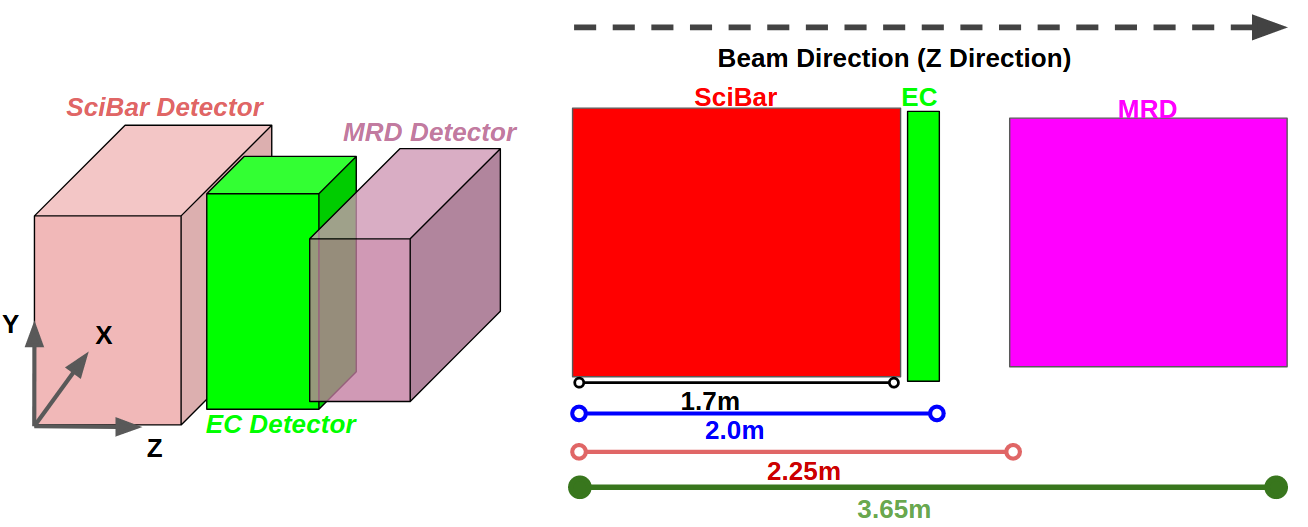
\includegraphics[width=0.75\textwidth]{EventClassifications/SciBooNEDetector.png}
\caption*{Figure \ref*{fig:SciBooNEDetector}: Representation of the SciBooNE detector and the coordinate frame we use in this study}
\end{figure}\label{fig:SciBooNEDetector}

%----------------------------------------------------------------------|
\subsubsection{The Scintillator Bar Tracker (SciBar)} \label{subsubsec:SciBar}
%----------------------------------------------------------------------|
The Scintillator Bar Tracker (SciBar) sub-detector is a scintillator detector which was used to identify neutrino interactions within SciBooNE. The dimensions of the SciBar detector used in this simulation are $0 < x < 3.0$ m, $0 < y < 3.0$ m, and $0 < z < 1.7$ m. This simulation models the scintillator materials as having a constant energy deposition per unit length ($dE/dx$) for both muons and pions of $2.04$ MeV/cm based on previous SciBooNE analyses and on mean values for typical particle momentum in the PDG.

%----------------------------------------------------------------------|
\subsubsection{The Muon Range Detector (MRD)}\label{subsubsec:MRD}
%----------------------------------------------------------------------|
The Muon Range Detector (MRD), depicted in Figure \ref*{fig:mrddetector} is located $0.55$ $m$ downstream of SciBar in the z-direction, and is a composition of two sets of thirteen alternating slabs of steel-scintillator layers, where the scintillator layers alternate between being horizontally oriented or vertically oriented, in the $xy$-plane. The steel layers have a z-direction thickness of $5.08$ $cm$ and the scintillator layers have a z-direction thickness of $0.6$ $cm$. Combining all the layers of the different alternating materials results in 26 scintillator layers that "sandwich" twenty five steel layers in-between and gives a total z-direction dimension of being $1.37 m$. The xy-plane is modeled as a square again (as was the case with SciBar, too) with dimensions in the x-direction and the y-direction of $2.6$ $m$. The energy deposition per unit length ($dE/dx$) of a muon penetrating the scintillator layers is assumed to be a constant $2.04$ MeV/cm while the energy deposition for the muon in the steel layers is assumed to be a greater value of $11.43$ $MeV/cm$. Both values are typical for muons at the energy range produced in SciBooNE and taken from the PDG.

\begin{figure}[H]
\centering
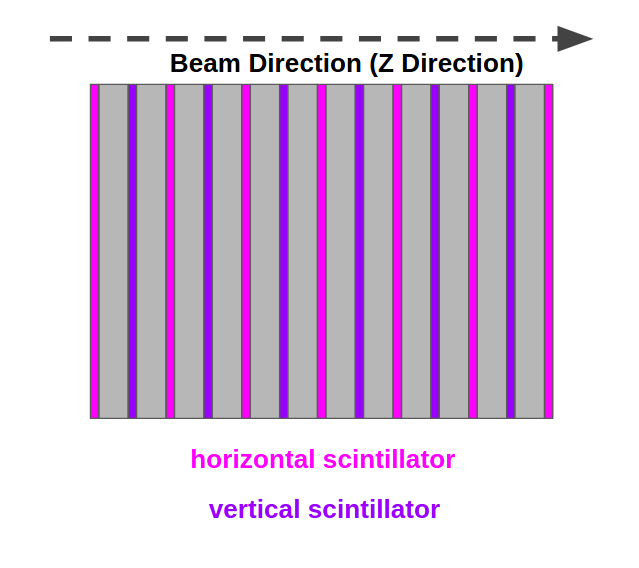
\includegraphics[width=0.75\textwidth]{EventClassifications/mrd.png}
\caption*{Figure \ref*{fig:mrddetector}: Depiction of the Muon Range Detector (MRD) which consists of alternating layers of horizontal scintillator (shown in pink) steel slabs (shown in grey) and vertical scintillator (shown in purple)}
\end{figure}\label{fig:mrddetector}



%=======================================================================
\section{Event Selection}\label{sec:eventselection}
%=======================================================================
Two main samples are used in this study to generate the acceptance tables. The first is a charged current inclusive (CC-Inclusive) sample which requires a muon was created in the neutrino interaction and this muon intersects the MRD. This sample is described in Section \ref*{sub:CCInclusive}.

The second sample is the charged current coherent pion (CC-Coh $\pi^{+/-}$) sample which requires a muon and charged pion are created in the neutrino interaction exclusively (e.g. no other final state particles in the event). This sample is described in Section \ref*{sub:CCCohPion}.

Both of these samples are selected using NEUT MC-truth flags which ensure we are treating pure samples which are classified by the neutrino generator as belonging to the appropriate sample.

Whether or not the event identified by our selection makes it into the final sample used in the acceptance study depends on the behavior of the muon with respect to the MRD. A muon which enters the MRD from a neutrino interaction will either come to stop in the MRD, exit out the back of the MRD (assuming it's momentum is great enough), or exit out the side of the MRD. In the next sections we explain this classification further.

%----------------------------------------------------------------------|
\subsection{Muon Stops within the MRD (``Stopped'')}\label{subsec:stoppedMRD}
%----------------------------------------------------------------------|
The requirement to classify a neutrino interaction as a ``stopped'' event requires the muon from the interaction to have reached the MRD, penetrated at least three layers of steel (giving activity in three layers of scintillator), and to then deposit all of its remaining energy prior to reaching a boundary of the MRD. An illustration of a CC-Coh $\pi^{+/-}$ event which would be classified as ``stopped'' is shown in Figure \ref*{fig:stoppedEvent}.

\begin{figure}[H]
\centering
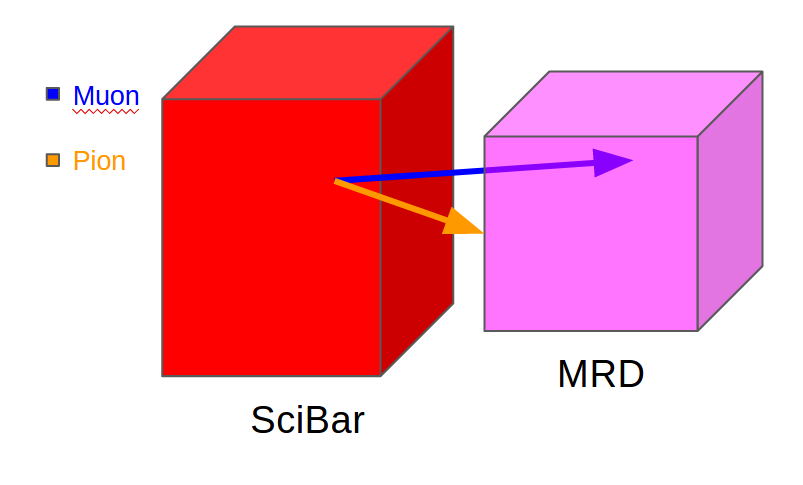
\includegraphics[width=0.6\textwidth]{EventClassifications/Stopped.png}
\caption*{Figure \ref*{fig:stoppedEvent}: Depiction of an event that was classified as "Stopped."}
\end{figure}\label{fig:stoppedEvent}

These events allow for complete reconstruction of the muon's momentum based on the number of layers which the muon penetrated and the muons incident angle.

%----------------------------------------------------------------------|
\subsection{Muon exits out the back of the MRD (``Out-the-back'')}
%----------------------------------------------------------------------|
The classification of a neutrino interaction as ``out-the-back'' requires that the muon from the interaction to have reached the MRD and to have had sufficient kinematics to have exited out the back face of the MRD without stopping. An illustration of such an event is given in Figure \ref*{fig:NotStoppedEvent}. 

\begin{figure}[H]
\centering
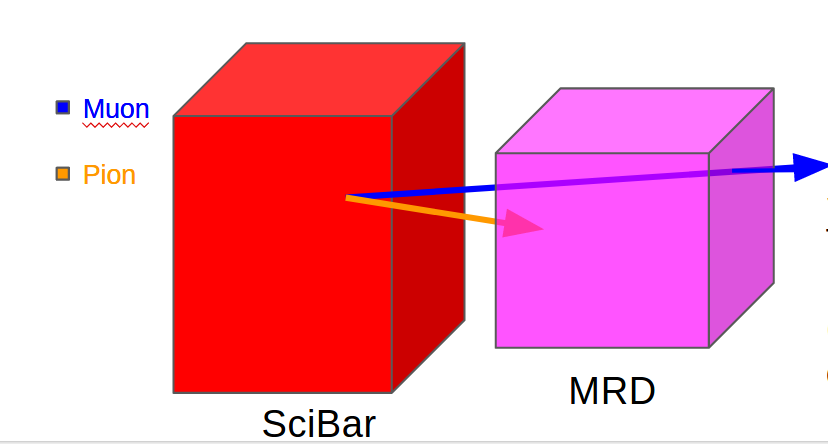
\includegraphics[width=0.6\textwidth]{EventClassifications/NotStopped.png}
\caption*{Figure \ref*{fig:NotStoppedEvent}: Depiction of an event that was classified as ``out-the-back''.}
\end{figure}\label{fig:NotStoppedEvent}

The exact momentum of muons which pass completely through the MRD could not be made in reconstruction, so these events were classified as having the minimum energy required to penetrate all the steel and scintillator layers of the MRD.

%----------------------------------------------------------------------|
\subsection{Muon exits out the side of the MRD (``Out-the-side'')}
%----------------------------------------------------------------------|
The classification of a neutrino interaction as ``out-the-side'' requires that the muon from the interaction reached the MRD, penetrated at least three layers of steel, and then to have exited out the side of the active volume of the MRD (excluding the very back face). Events which are classified as ``out-the-side'' are excluded from this study because no accurate reconstruction of the muons momentum can be made when the muon exits out the side of the MRD. An illustration of such an excluded event which exits out the side of the MRD is given in Figure \ref*{fig:OutTheSideEvent}.


\begin{figure}[H]
\centering
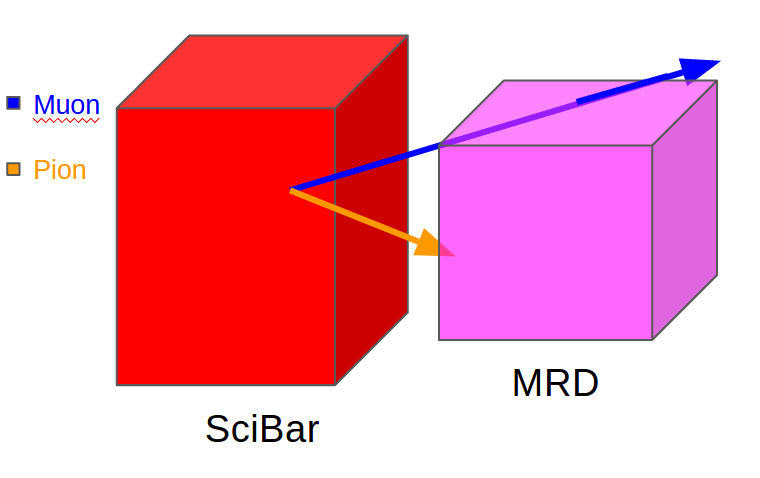
\includegraphics[width=0.6\textwidth]{EventClassifications/OutSide.png}
\caption*{Figure \ref*{fig:OutTheSideEvent}: Depiction of an event that was classified as "Out-Side."}
\end{figure}\label{fig:OutTheSideEvent}




%=======================================================================
\section{Results}\label{sec:Results}
%=======================================================================
The results of this acceptance study can be broken down into two different classification schemes of events. Those that met the conditions to qualify as a CC-Inclusive event, and those that met the conditions of classification as Charged-Current Coherent Pion Production events. The plots in the two subsections below show our results.

%---------------------------------------------------------------------|
\subsection{Charged-Current Inclusive Events}\label{sub:CCInclusive}
%---------------------------------------------------------------------|

Here we define the charged current inclusive sample (CC-Inclusive) which we use to validate our acceptance model against previous simulation studies which were done. Table \ref*{tab:NuCCIncEventReduction} goes through the event selection criteria for selecting a sample of CC-Inclusive events from the neutrino mode ($\nu$-mode) Monte Carlo.

\begin{center}
\begin{table}[htb]
	\begin{center}
	\resizebox{0.99\textwidth}{!}{%
	\begin{tabular}{|c|c|c|c|}
	\multicolumn{4}{c}{\textbf{$\nu$-mode CC-Inclusive Event Reduction}} \\
	\hline \hline
	 Events Selection & NEUT v5.3.6 Rein-Sehgal & NEUT v5.3.6 Berger-Sehgal & NEUT vx.x.x Rein-Sehgal\\
	\hline
	 Total Sample & 1,000,000 & 1,000,000 & 100,000 \\
	\hline
	CC-Inclusive Interaction & 725,730 & 727,278 & 69,363 \\
	($\mu$ + n-other particles in SciBar) & & & \\
	\hline
	Muon enters the MRD & 263,698 & 262,608 & 24,250 \\
	\hline
	Muon enters the MRD and & 231,089 & 230,054 & 21,001 \\
	penetrates $\geq$ 3 layers of steel & & & \\
	\hline
	``Stopped''-Events & 177,406 & 175,799 & 16,062 \\
	``Out-the-back''-Events & 15,389 & 15,952 & 1,421 \\
	``Out-the-side''-Events & 38,294 & 38,303 & 3,518 \\
	\hline
	\hline
	\textbf{Good CC-Inclusive Events} & \textbf{192,795} & \textbf{191,751} & \textbf{17,483} \\
	\hline
	\hline
	\end{tabular}}
	\caption*{Table \ref*{tab:NuCCIncEventReduction}: Event reduction table for a sample of $\nu$-mode CC-Inclusive events simulated in the SciBooNE geometry.}
	\end{center}
\end{table}\label{tab:NuCCIncEventReduction}
\end{center}

Figure \ref*{fig:NuModeCCInclusiveMomAndAng} shows the momentum and angular distribution for the sample of $\nu$-mode CC-Inclusive events passing all our requirements for all three models considered in this study (NEUT v5.3.6 Rein-Sehgal, NEUT v5.3.6 Berger-Sehgal, NEUT vx.x.x Rein-Sehgal). The distributions have been normalized to the same area and show no strong differences between them.


\begin{figure}[H]
\centering
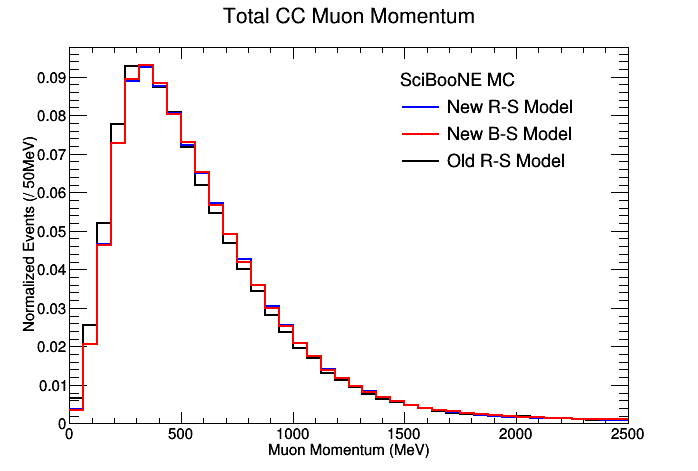
\includegraphics[width=0.4\textwidth]{CCInclusivePlots/NMCCInclusiveTotalMomentum.png}
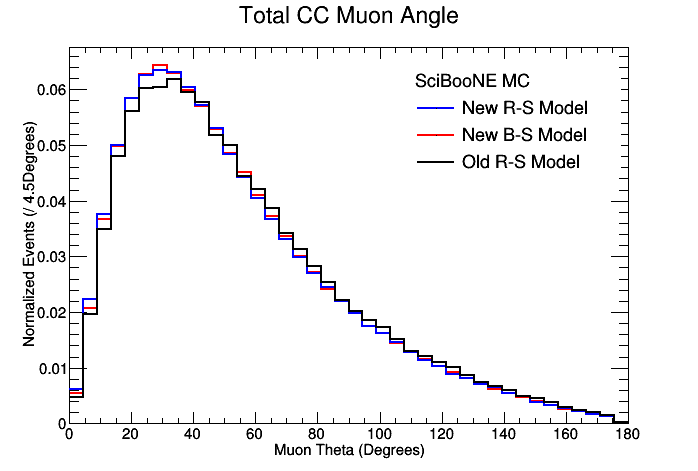
\includegraphics[width=0.4\textwidth]{CCInclusivePlots/NMCCInclusiveTotalAngle.png}
\caption*{Figure \ref*{fig:NuModeCCInclusiveMomAndAng}: Muon Momentum (left) and Muon Angle (right) for $\nu$-mode CC-Inclusive interactions for all three models included in this study. These samples kinematics are, unsurprisingly, very similar for the sample of CC-Inclusive}
\end{figure}\label{fig:NuModeCCInclusiveMomAndAng}


Figure \ref*{fig:OneDEfficiency} represents the one-dimensional efficiency for selecting $\nu$-mode CC-Inclusive events for this study compared to results derived from Hirade's thesis (need proper reference) using the full SciBooNE Monte Carlo simulation. A few reference points are illustrated using dashed lines to guide the readers eye. A few perecent difference is seen, but overall agreement between the two simulations hold. 

\begin{figure}[H]
\centering
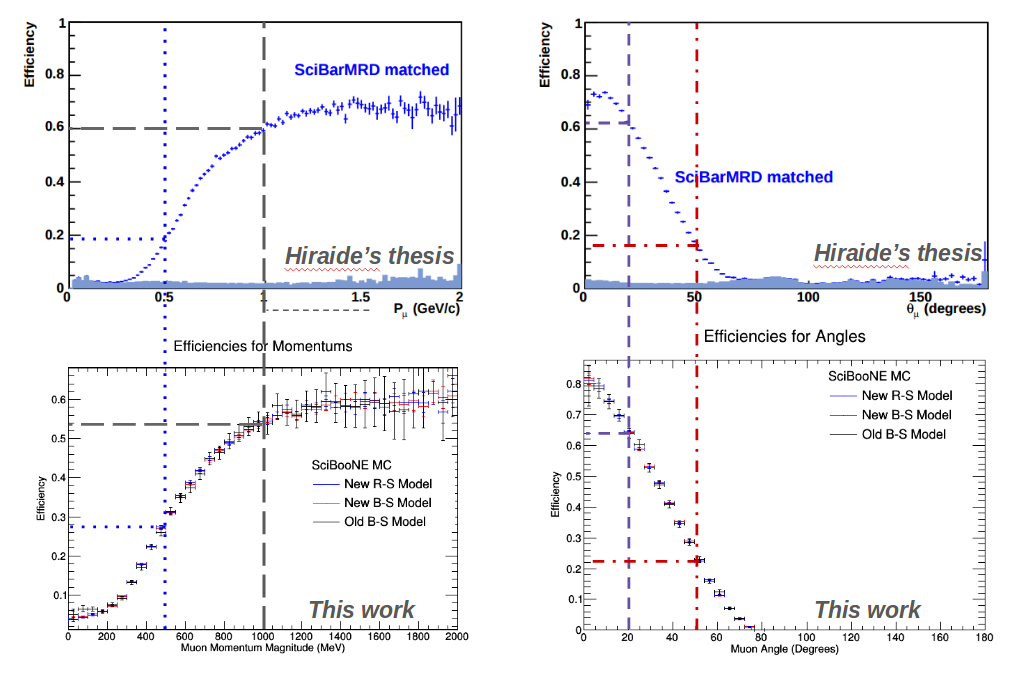
\includegraphics[width=0.8\textwidth]{CCInclusivePlots/CCInc1DEff.png}
\caption*{Figure \ref*{fig:OneDEfficiency}: One-dimension efficiency plots for the $\nu$-mode CC-Inclusive sample.}
\end{figure}\label{fig:OneDEfficiency}


Figure \ref*{fig:TwoDEfficiencyRS} shows the two-dimensional efficiency for selecting $\nu$-mode CC-Inclusive events for this study compared to results derived from Morgan's reference sample (need more words here about this....see email)

\begin{figure}[H]
\centering
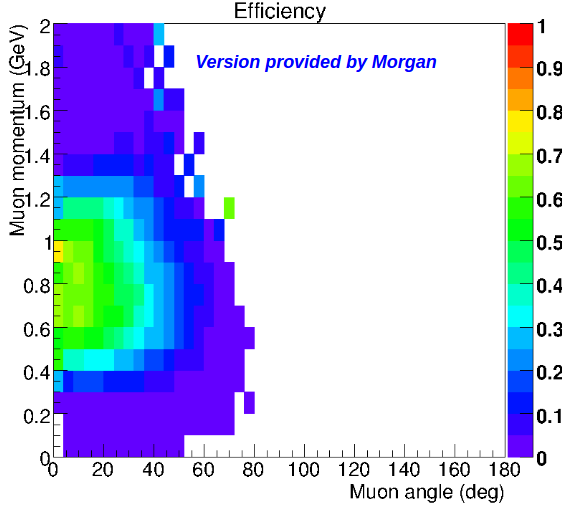
\includegraphics[width=0.3\textwidth]{CCInclusivePlots/MorgansCCInclusiveSample.png}
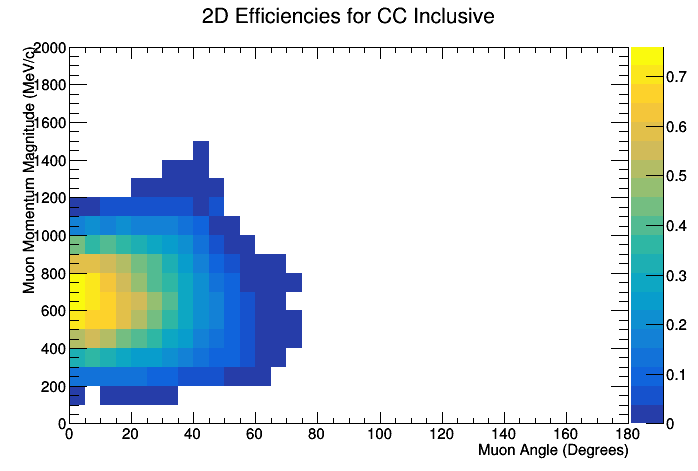
\includegraphics[width=0.4\textwidth]{CCInclusivePlots/2DEffCompareNMRS.png}
\caption*{Figure \ref*{fig:TwoDEfficiencyRS}: Two-dimensional efficiency plots for the $\nu$-mode Rein-Sehgal CC-Inclusive sample.}
\end{figure}\label{fig:TwoDEfficiencyRS}

\begin{figure}[H]
\centering
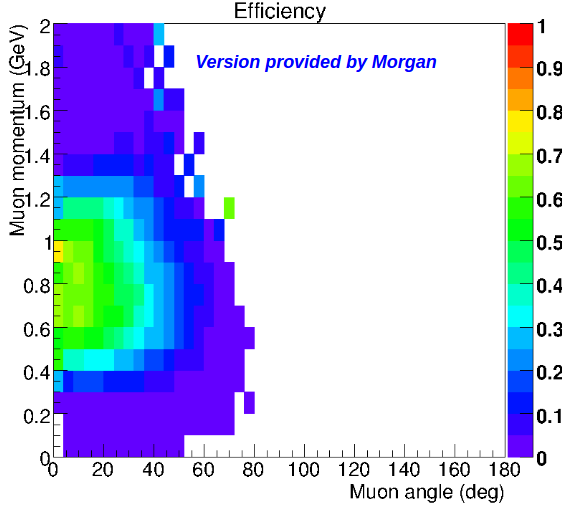
\includegraphics[width=0.3\textwidth]{CCInclusivePlots/MorgansCCInclusiveSample.png}
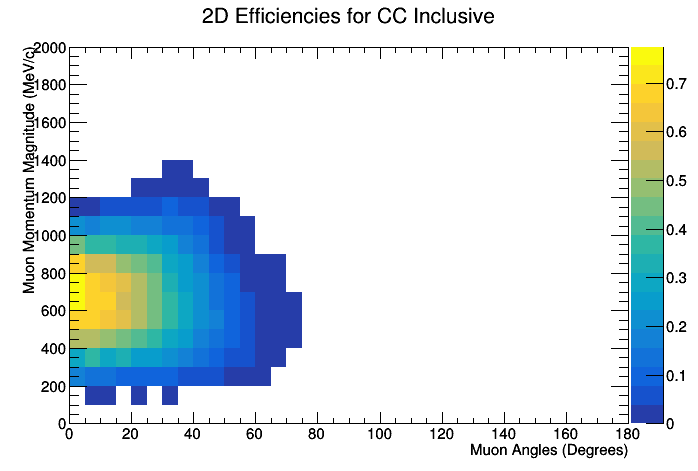
\includegraphics[width=0.4\textwidth]{CCInclusivePlots/2DEffCompareNMBS.png}
\caption*{Figure \ref*{fig:TwoDEfficiencyBS}: Two-dimensional efficiency plots for the $\nu$-mode Berger-Sehgal CC-Inclusive sample.}
\end{figure}\label{fig:TwoDEfficiencyBS}

\begin{figure}[H]
\centering
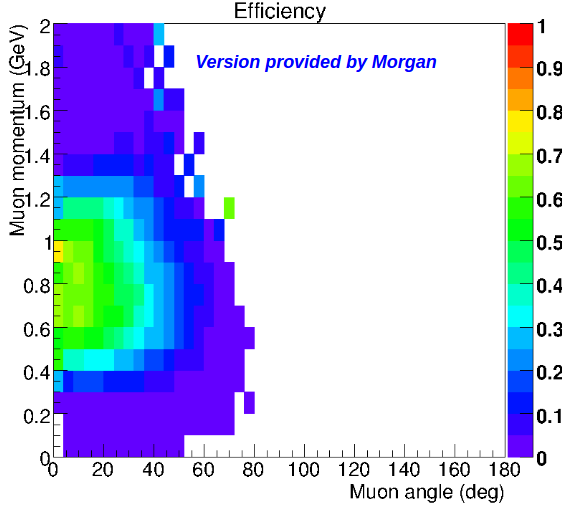
\includegraphics[width=0.3\textwidth]{CCInclusivePlots/MorgansCCInclusiveSample.png}
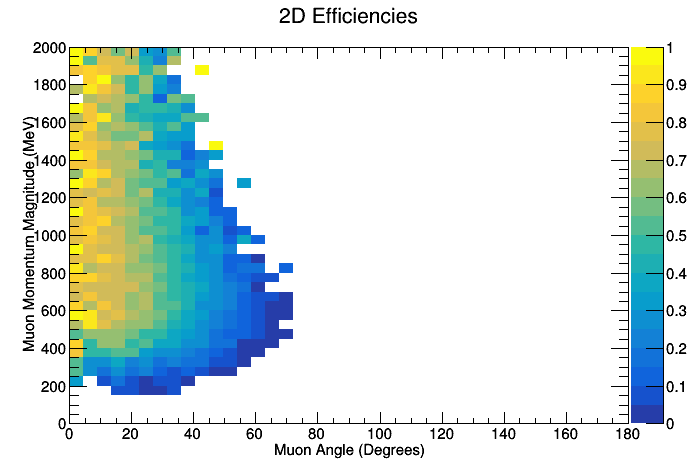
\includegraphics[width=0.4\textwidth]{CCInclusivePlots/2DEffCompareNMORS.png}
\caption*{Figure \ref*{fig:TwoDEfficiencyORS}: Two-dimensional efficiency plots for the $\nu$-mode Old Rein-Sehgal CC-Inclusive sample.}
\end{figure}\label{fig:TwoDEfficiencyORS}

Similar to before, Table \ref*{tab:AntiNuCCIncEventReduction} goes through the event selection criteria for selecting a sample of CC-Inclusive events from the neutrino mode ($\bar{\nu}$-mode) Monte Carlo.


\begin{center}
\begin{table}[htb]
	\begin{center}
	\resizebox{0.99\textwidth}{!}{%
	\begin{tabular}{|c|c|c|}
	\multicolumn{3}{c}{\textbf{$\bar{\nu}$-mode CC-Inclusive Event Reduction}} \\
	\hline \hline
	 Events Selection & NEUT v5.3.6 Rein-Sehgal & NEUT v5.3.6 Berger-Sehgal \\
	\hline
	 Total Sample & 1,000,000 & 1,000,000 \\
	\hline
	CC-Inclusive Interaction & 699,239 & 704,327 \\
	($\mu$ + n-other particles in SciBar) & & \\
	\hline
	Muon enters the MRD & 380,362 & 380,869 \\
	\hline
	Muon enters the MRD and & 336,373 & 337,979 \\
	penetrates $\geq$ 3 layers of steel & & \\
	\hline
	``Stopped''-Events & 288,289 & 288,206 \\
	``Out-the-back''-Events & 7,608 & 7,857 \\
	``Out-the-side''-Events & 40,476 & 41,916 \\
	\hline
	\hline
	\textbf{Good CC-Inclusive Events} & \textbf{295,897} & \textbf{296,063} \\
	\hline
	\hline
	\end{tabular}}
	\caption*{Table \ref*{tab:AntiNuCCIncEventReduction}: Event reduction table for a sample of $\bar{\nu}$-mode CC-Inclusive evnets simulated in the SciBooNE geometry.} 
	\end{center}
\end{table}\label{tab:AntiNuCCIncEventReduction}
\end{center}


Figure \ref*{fig:NuModeCCInclusiveMomAndAng} shows the momentum and angular distribution for the sample of $\bar{\nu}$-mode CC-Inclusive events passing all our requirements for all three models considered in this study (NEUT v5.3.6 Rein-Sehgal, NEUT v5.3.6 Berger-Sehgal, NEUT vx.x.x Rein-Sehgal). The distributions have been normalized to the same area and show no strong differences between them. 

\begin{figure}[H]
\centering
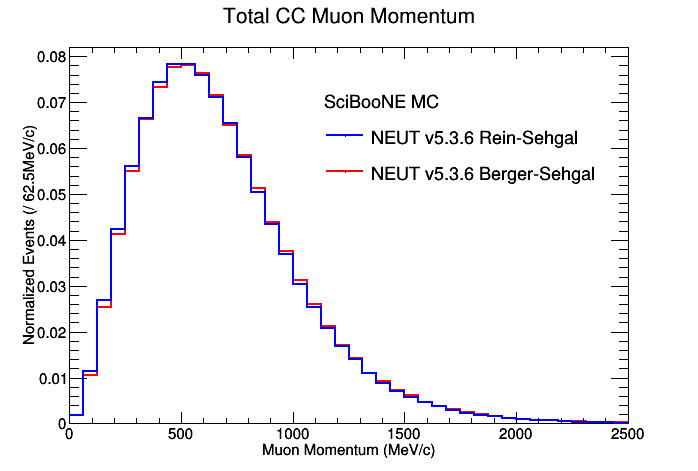
\includegraphics[width=0.4\textwidth]{CCInclusivePlots/ANMCCInclusiveTotalMomentum.png}
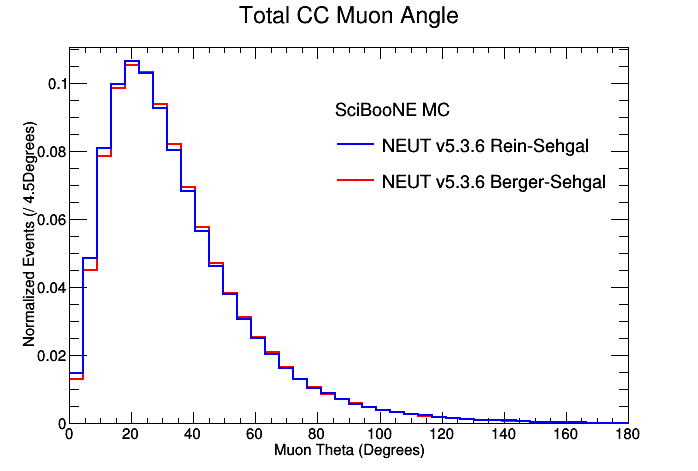
\includegraphics[width=0.4\textwidth]{CCInclusivePlots/ANMCCInclusiveTotalAngle.png}
\caption*{Figure \ref*{fig:AntiNuCCInclusiveMomAndAngle}: Muon Momentum (left) and Muon Angle (right) for $\bar{\nu}$-mode CC-Inclusive interactions for all three models included in this study. These samples kinematics are, unsurprisingly, very similar for the sample of CC-Inclusive}
\end{figure}\label{fig:AntiNuCCInclusiveMomAndAngle}

Figure \ref*{fig:OneDEfficiencyAntiNu} represents the one-dimensional efficiency for selecting $\bar{\nu}$-mode CC-Inclusive events for this study. No similar reference sample exists to be compared directly against, however we note that the shape and magnitude of the acceptance is nearly unchanged between $\bar{\nu}$ and $\nu$-mode samples (as expected).

\begin{figure}[H]
\centering
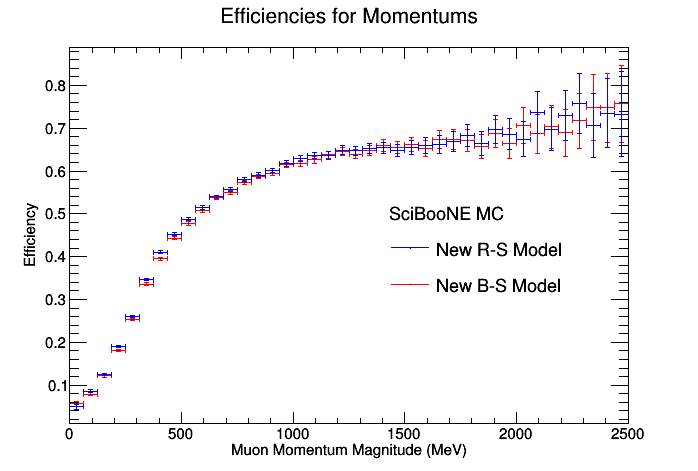
\includegraphics[width=0.4\textwidth]{CCInclusivePlots/OneDAntiNuEffMomentum.png}
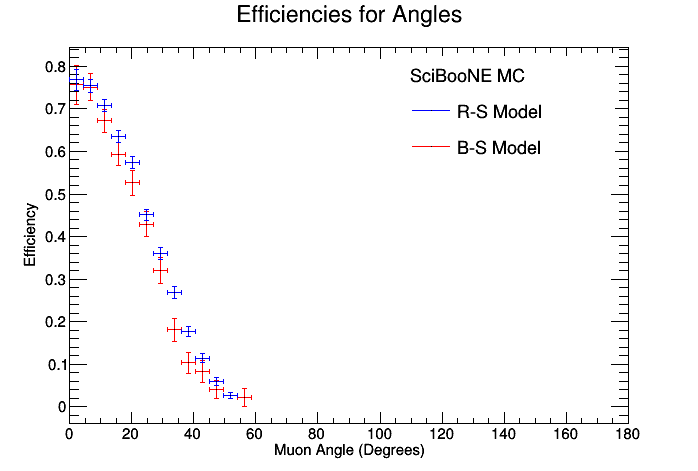
\includegraphics[width=0.4\textwidth]{CCInclusivePlots/OneDAntiNuEffAngle.png}
\caption*{Figure \ref*{fig:OneDEfficiencyAntiNu}: One-dimension efficiency plots for the $\bar{\nu}$-mode CC-Inclusive sample. Muon's Momentums is on the right and the Muon's Angles is on the left.}
\end{figure}\label{fig:OneDEfficiencyAntiNu}

Figure \ref*{fig:TwoDEfficiencyRS} shows the two-dimensional efficiency for selecting $\bar{\nu}$-mode CC-Inclusive events for this study compared to results derived from Morgan's reference sample (need more words here about this....see email)

\begin{figure}[H]
\centering
%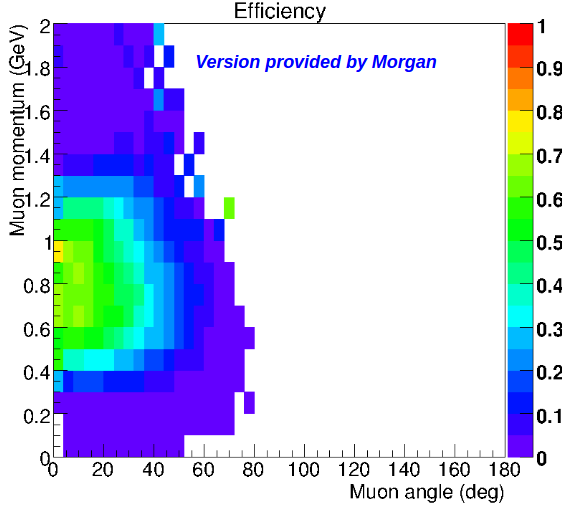
\includegraphics[width=0.3\textwidth]{CCInclusivePlots/MorgansCCInclusiveSample.png}
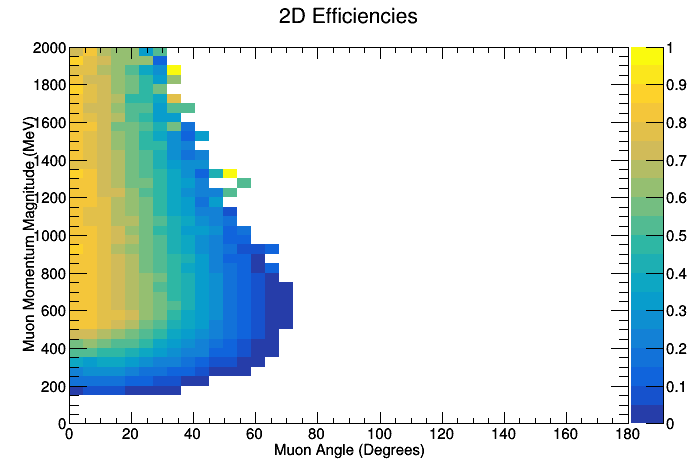
\includegraphics[width=0.6\textwidth]{CCInclusivePlots/2DEffCompareANMRS.png}
\caption*{Figure \ref*{fig:TwoDEfficiencyRS}: Two-dimensional efficiency plot for the $\bar{\nu}$-mode Rein-Sehgal CC-Inclusive sample.}
\end{figure}\label{fig:TwoDEfficiencyRS}

\begin{figure}[H]
\centering
%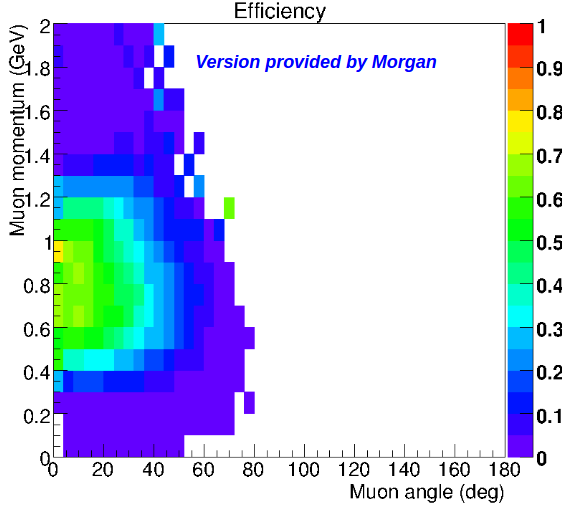
\includegraphics[width=0.3\textwidth]{CCInclusivePlots/MorgansCCInclusiveSample.png}
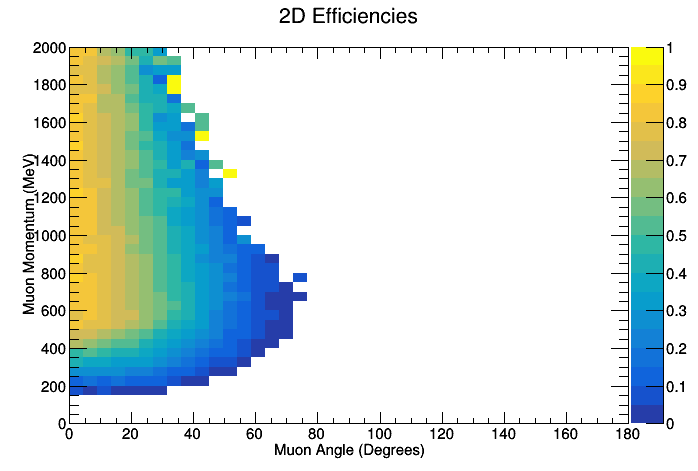
\includegraphics[width=0.6\textwidth]{CCInclusivePlots/2DEffCompareANMBS.png}
\caption*{Figure \ref*{fig:TwoDEfficiencyBS}: Two-dimensional efficiency plot for the $\bar{\nu}$-mode Berger-Sehgal CC-Inclusive sample.}
\end{figure}\label{fig:TwoDEfficiencyBS}

Below are the tables that correspond to the five 2D Efficiency CC-Inclusive histograms that are above.

% Here are the tables for the 2D efficiency histograms
\newpage
\begin{landscape}
\begin{table}
\centering
\caption{Table for 2D Histogram for New NM-Rein-Sehgal}
\begin{adjustbox}{width=\paperwidth}
\csvautotabular{TechNoteTables/New-NM-RS.csv}
\end{adjustbox}
\end{table}
\end{landscape}

\newpage
\begin{landscape}
\begin{table}
\centering
\caption{Table for 2D Histogram for New NM-Berger-Sehgal}
\begin{adjustbox}{width=\paperwidth}
\csvautotabular{TechNoteTables/New-NM-BS.csv}
\end{adjustbox}
\end{table}
\end{landscape}

\newpage
\begin{landscape}
\begin{table}
\centering
\caption{Table for 2D Histogram for Old NM-Rein-Sehgal}
\begin{adjustbox}{width=\paperwidth}
\csvautotabular{TechNoteTables/Old-NM-RS.csv}
\end{adjustbox}
\end{table}
\end{landscape}

\newpage
\begin{landscape}
\begin{table}
\centering
\caption{Table for 2D Histogram for New ANM-Rein-Sehgal}
\begin{adjustbox}{width=\paperwidth}
\csvautotabular{TechNoteTables/New-ANM-RS.csv}
\end{adjustbox}
\end{table}
\end{landscape}

\newpage
\begin{landscape}
\begin{table}
\centering
\caption{Table for 2D Histogram for New ANM-Berger-Sehgal}
\begin{adjustbox}{width=\paperwidth}
\csvautotabular{TechNoteTables/New-ANM-BS.csv}
\end{adjustbox}
\end{table}
\end{landscape}
% This is where the 2D efficiency histograms end



%---------------------------------------------------------------------|
\subsection{Charged-Current Coherent Pion Production Events}\label{sub:CCCohPion}
%---------------------------------------------------------------------|

Here we define the Charged-Current Coherent Pion Production sample (CC-Coh $\pi^{+/-}$) which we use to validate our acceptance model against previous simulation studies which were done. Table \ref{tab:NuCCCoherentEventReduction} goes through the event selection criteria for selecting a sample of CC-Coh $\pi^{+/-}$ events from the neutrino mode ($\nu$-mode) Monte Carlo.

\begin{center}
\begin{table}[htb]
	\begin{center}
	\resizebox{0.99\textwidth}{!}{%
	\begin{tabular}{|c|c|c|c|}
	\multicolumn{4}{c}{\textbf{$\nu$-mode CC-Coherent Pion Event Reduction}} \\
	\hline \hline
	 Events Selection & NEUT v5.3.6 Rein-Sehgal & NEUT v5.3.6 Berger-Sehgal & NEUT vx.x.x Rein-Sehgal\\
	\hline
	Total Sample & 1,000,000 & 1,000,000 & 100,000 \\
	\hline
	CC-Coherent Pion Interaction & 12,186 & 2,576 & 1,320 \\
	($\mu$ + $\pi$ + $\varnothing$ in SciBar) & & & \\
	\hline
	Both muon and pion are  & 8,535 & 1,845 & 884 \\
	forward going &  &  &  \\
	\hline
	Muon enters the MRD and & 7,407 & 1,592 & 767 \\
	penetrates $\geq$ 3 layers of steel & & & \\
	\hline
	``Stopped''-Events & 6,448 & 1,350 & 669 \\
	``Out-the-back''-Events & 530 & 150 & 56 \\
	``Out-the-side''-Events & 429 & 92 & 42 \\
	\hline
	\hline
	\textbf{Good Coherent Pion Events} & \textbf{6,978} & \textbf{1,500} & \textbf{725} \\
	\hline
	\hline
	\end{tabular}}
	\caption{Event reduction table for a sample of $\nu$-mode Charged Current Coherent Pion events simulated in the SciBooNE geometry.} 
	\end{center}
\end{table}\label{tab:NuCCCoherentEventReduction}
\end{center}

% YOU NEED TO RE-WRITE WHAT IS BETWEEN HERE--
The NewANMBergerSehgal.C macro also calculates many different quantities for the generated simulation of the events and saves the information in histograms that are later called upon through the plotting macros (which are after all of the analysis macros). The first quantity that is calculated for the different vertexes is the momentum of both the muon and the pion, which are both calculated using the equations:

\begin{equation}
|\vec{p}_\mu| = \sqrt{P_{\mu_x}^2 + P_{\mu_y}^2 + P_{\mu_z}^2}
\end{equation}

\begin{equation}
|\vec{p}_\pi| = \sqrt{P_{\pi_x}^2 + P_{\pi_y}^2 + P_{\pi_z}^2}
\end{equation}

\noindent
The momentum is reported in units of $MeV/c$.

The next quantity that is calculated in the macro is the angle from the beam-direction for both the muon and the pion, which are labeled as either $\theta_\mu$, or $\theta_\pi$, respectively. The angle from the beam-direction is the same as the angle from the z-direction, and this angle is known as the azimuthal angle. The calculation of the azimuthal angle is slightly more involved than the simple calculation used for finding the magnitude of the momentum of the two particles, and is calculated using the equations:

\begin{equation}
\theta_\mu = tan^{-1}\Bigg(\frac{\sqrt{P_{\mu_x}^2 + P_{\mu_y}^2}}{P_{\mu_z}}\Bigg)
\end{equation}

\begin{equation}
\theta_\pi = tan^{-1}\Bigg(\frac{\sqrt{P_{\pi_x}^2 + P_{\pi_y}^2}}{P_{\pi_z}}\Bigg)
\end{equation}

\noindent
The angles are reported in units of $\degree$, and should run from $0\degree$ to $180\degree$. In the case of charged-current coherent pion production, the angle should never be larger than $90\degree$.
% --AND HERE!!


\begin{figure}[H]
\centering
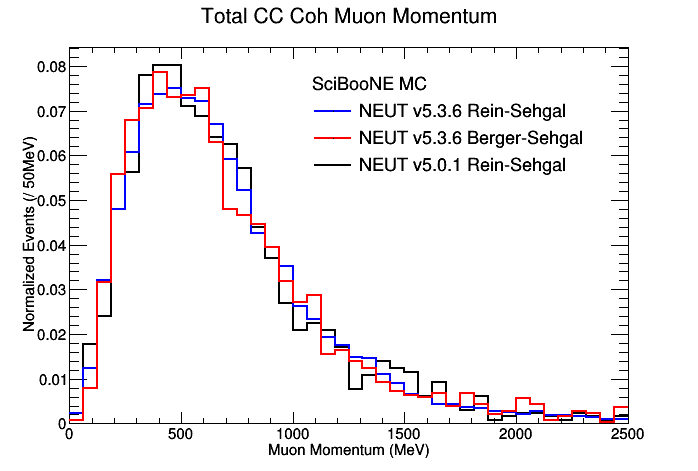
\includegraphics[width=0.4\textwidth]{CCCohPlots/NMCCCohTotalMomentum.png}
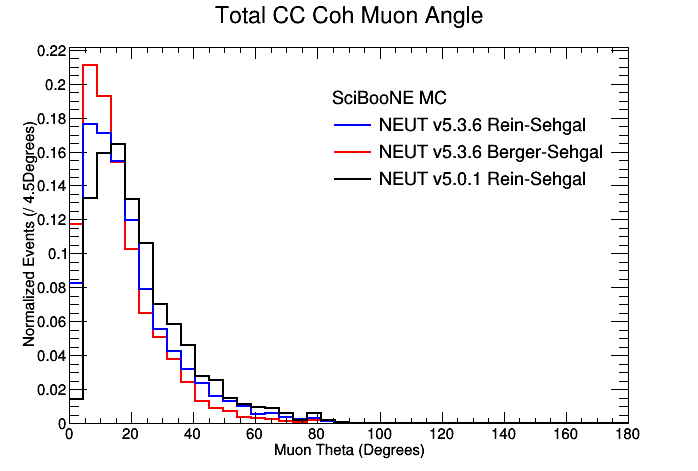
\includegraphics[width=0.4\textwidth]{CCCohPlots/NMCCCohTotalAngle.png}
\caption{"Total" Muon Momentum (left) and "Total" Muon Angle (right) for $\nu$-mode CC-Coh $\pi^{+/-}$ interactions for all three models included in this study. The "Total" classification means that all CC-Coh $\pi^{+/-}$ events are included in these histograms.}
\end{figure}\label{fig:NuModeCCCohTotalMomAndAng}

Here will be the plots for CC-Coh Pion with the good momentum efficiencies and the angle efficiencies!

\begin{figure}[H]
\centering
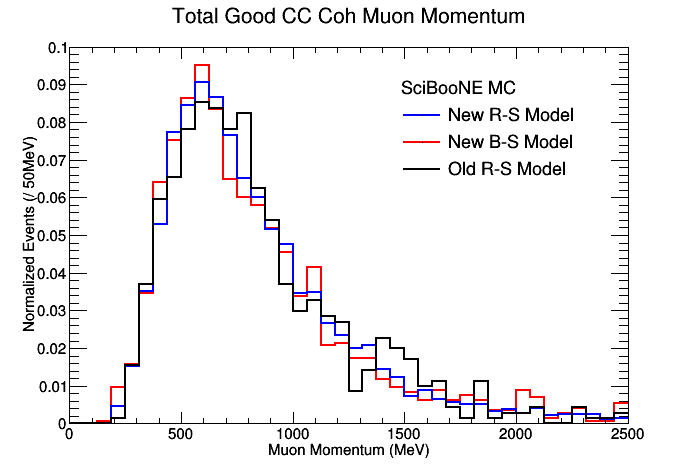
\includegraphics[width=0.4\textwidth]{CCCohPlots/NMCCCohGoodMomentum.png}
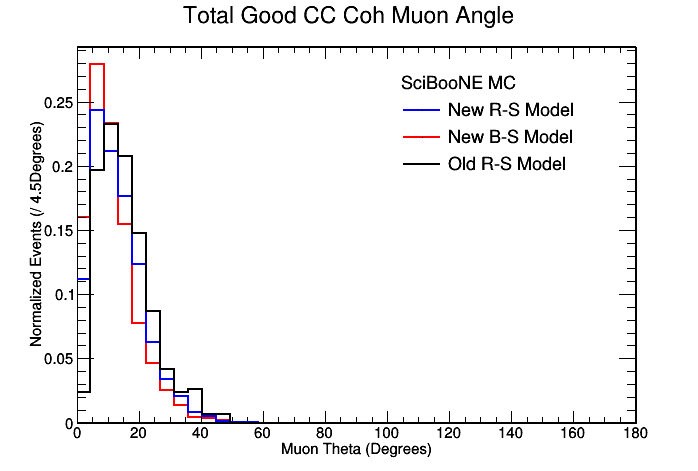
\includegraphics[width=0.4\textwidth]{CCCohPlots/NMCCCohGoodAngle.png}
\caption{"Good" Muon Momentum (left) and "Good" Muon Angle (right) for $\nu$-mode CC-Coh $\pi^{+/-}$ interactions for all three models included in this study. The "Good" classification means that only the stopped and not-stopped CC-Coh $\pi^{+/-}$ events are included for these histograms.}
\end{figure}\label{fig:NuModeCCCohGoodMomAndAng}

Now from here on will be the rest of the results for CC-Coh Events (so this will be the $|t|$ and $Q^2$ plots with the explanations for what they are!!). You might also want to make a figure that depicts what the $\theta_{particle}$'s are... think about it.

% You need to rewrite what is between here, but these equations are correct!
The last two quantities that this analysis macro calculates are the two different types of four-momentum transfers specific to this interaction, which are $Q^2$ and $|t|$. The $Q^2$ corresponds to the four-momentum transfer from the neutrino and muon to the nucleus and pion, and is calculated using the equation:

\begin{equation}
Q^2 = |(P_{\nu_\mu} - P_\mu)^2|
\end{equation}

\noindent
This equation is the four-momentum notational form. The code follows the equation below in order to compute $Q^2$:

\begin{equation}
Q^2 = |(P_{\nu_{\mu,x}} - P_{\mu_x})^2 + (P_{\nu_{\mu,y}} - P_{\mu_y})^2 + (P_{\nu_{\mu,z}} - P_{\mu_z})^2 + (P_{\nu_{\mu,E}} - P_{\mu_E})^2|
\end{equation}

\noindent
$Q^2$ is reported in units of $(MeV/c)^2$.

The $|t|$ corresponds to the four-momentum transfer from the neutrino, muon, and pion to the nucleus, and is calculated using the equation:

\begin{equation}
|t| = |(Q - P_\pi)^2| = |(P_{\nu_\mu} - P_\mu - P_\pi)^2|
\end{equation}

\noindent
This equation is the four-momentum notational form. The code follows the equation below in order to compute $|t|$:

\begin{equation}
|t| = |(P_{\nu_{\mu,x}} - P_{\mu_x} - P_{\pi_x})^2 + (P_{\nu_{\mu,y}} - P_{\mu_y} - P_{\pi_y})^2 + (P_{\nu_{\mu,z}} - P_{\mu_z} - P_{\pi_z})^2 + (P_{\nu_{\mu,E}} - P_{\mu_E} - P_{\pi_E})^2|
\end{equation}

\noindent
$|t|$ is reported in units of $(MeV/c)^2$.
% And this is the end of the section that has been set aside with the intention of being rewritten

% This is where the t and q2 plots are
$\nu$-Mode $|t|$ and $Q^2$ plots are below:

\begin{figure}[H]
\centering
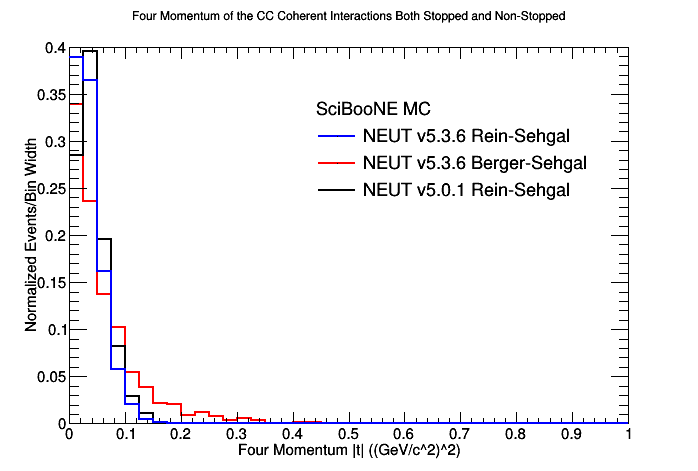
\includegraphics[width=0.4\textwidth]{CCCohPlots/NMCCCohGoodT.png}
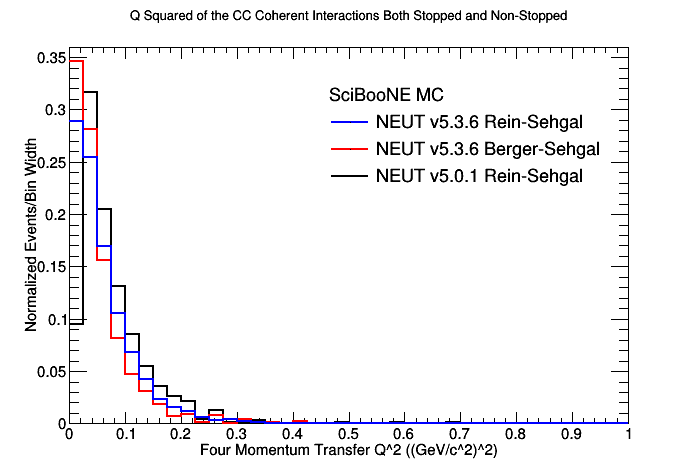
\includegraphics[width=0.4\textwidth]{CCCohPlots/NMCCCohGoodQ2.png}
\caption{The $|t|$ Good Momentum Transfer (left) and $Q^2$ Good Momentum Transfer (right) for $\nu$-mode CC-Coh $\pi^{+/-}$ interactions for the three models included in this study. The Good classification means that this includes both the stopped and the not-stopped classifications of the CC-Coh $\pi^{+/-}$ events only.}
\end{figure}\label{fig:AntiNuModeCCCohGoodTAndQ2}
%End of neutrino mode q2 and |t| plots!!



Similar to before, Table \ref{tab:AntiNuCCCoherentEventReduction} goes through the event selection criteria for selecting a sample of CC-Coh $\pi^{+/-}$ events from the neutrino mode ($\bar{\nu}$-mode) Monte Carlo.

\begin{center}
\begin{table}[htb]
	\begin{center}
	\resizebox{0.99\textwidth}{!}{%
	\begin{tabular}{|c|c|c|}
	\multicolumn{3}{c}{\textbf{$\bar{\nu}$-mode CC-Coherent Pion Event Reduction}} \\
	\hline \hline
	 Events Selection & NEUT v5.3.6 Rein-Sehgal & NEUT v5.3.6 Berger-Sehgal \\
	\hline
	Total Sample & 1,000,000 & 1,000,000 \\
	\hline
	CC-Coherent Pion Interaction & 36,669 & 7,790 \\
	($\mu$ + $\pi$ + $\varnothing$ in SciBar) & & \\
	\hline
	Both muon and pion are  & 24,675 & 5,477 \\
	forward going & & \\
	\hline
	Muon enters the MRD and & 20,445 & 4,517 \\
	penetrates $\geq$ 3 layers of steel & & \\
	\hline
	``Stopped''-Events & 18,935 & 4,203 \\
	``Out-the-back''-Events & 372 & 82 \\
	``Out-the-side''-Events & 1,138 & 232 \\
	\hline
	\hline
	\textbf{Good Coherent Pion Events} & \textbf{19,307} & \textbf{4,285} \\
	\hline
	\hline
	\end{tabular}}
	\caption{Event reduction table for a sample of $\bar{\nu}$-mode Charged Current Coherent Pion events simulated in the SciBooNE geometry.} 
	\end{center}
\end{table}\label{tab:AntiNuCCCoherentEventReduction}
\end{center}

Here will go the plots for CC-Coh Events for ANM both the momentums and the angles for total events.

\begin{figure}[H]
\centering
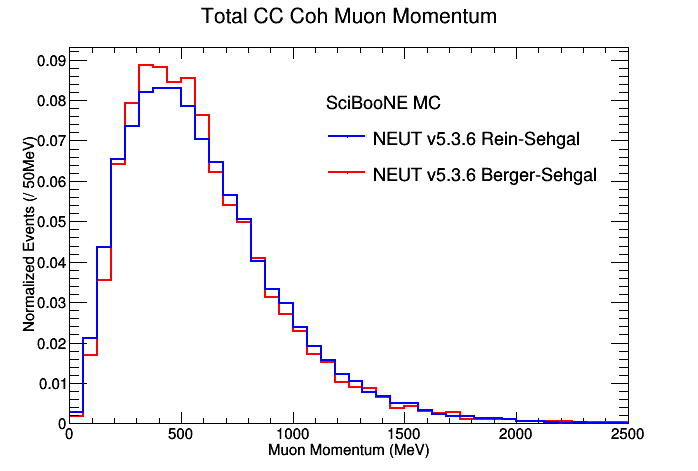
\includegraphics[width=0.4\textwidth]{CCCohPlots/ANMCCCohTotalMomentum.png}
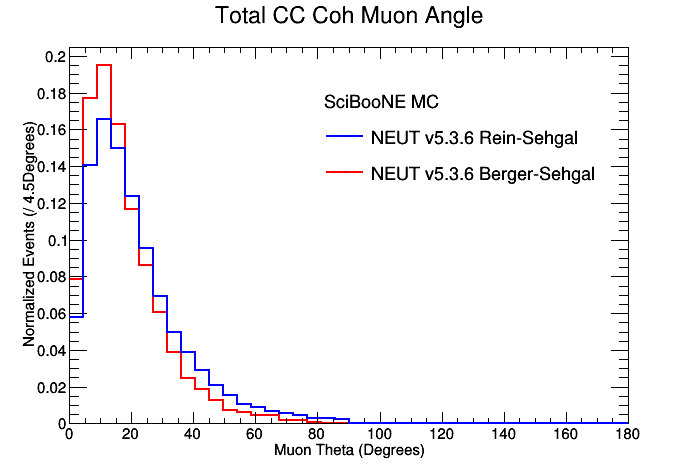
\includegraphics[width=0.4\textwidth]{CCCohPlots/ANMCCCohTotalAngle.png}
\caption{"Total" Muon Momentum (left) and "Total" Muon Angle (right) for $\nu$-mode CC-Coh $\pi^{+/-}$ interactions for all three models included in this study. The "Total" classification means that all CC-Coh $\pi^{+/-}$ events are included in these histograms.}
\end{figure}\label{fig:AntiNuModeCCCohTotalMomAndAng}

Here will go the plots for CC-Coh Events for ANM both the momentums and the angles for good events.

\begin{figure}[H]
\centering
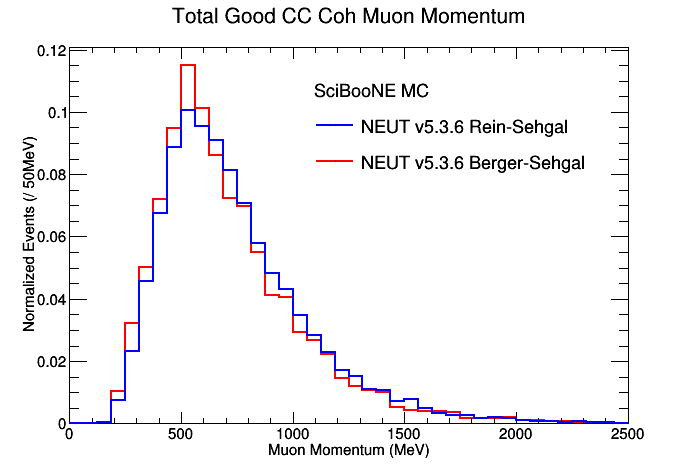
\includegraphics[width=0.4\textwidth]{CCCohPlots/ANMCCCohGoodMomentum.png}
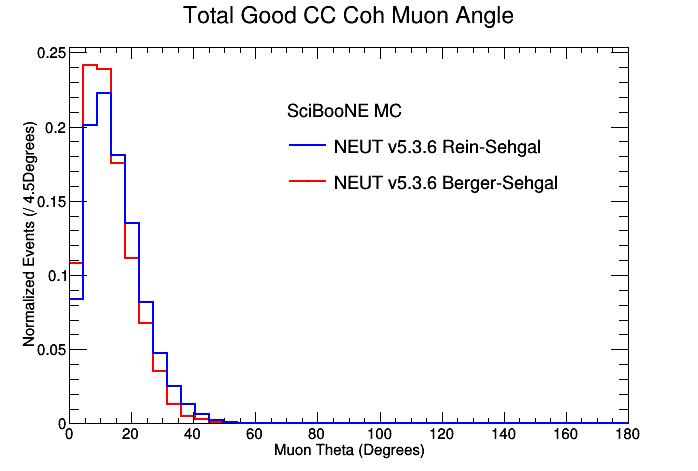
\includegraphics[width=0.4\textwidth]{CCCohPlots/ANMCCCohGoodAngle.png}
\caption{"Good" Muon Momentum (left) and "Good" Muon Angle (right) for $\bar{\nu}$-mode CC-Coh $\pi^{+/-}$ interactions for both of the models included in this study. The "Good" classification means that only the stopped and not-stopped CC-Coh $\pi^{+/-}$ events are included in these histograms.}
\end{figure}\label{fig:AntiNuModeCCCohGoodMomAndAng}

Here should be a description of the different t and q plots!

$\bar{\nu}$-Mode $|t|$ and $Q^2$ plots are below:

\begin{figure}[H]
\centering
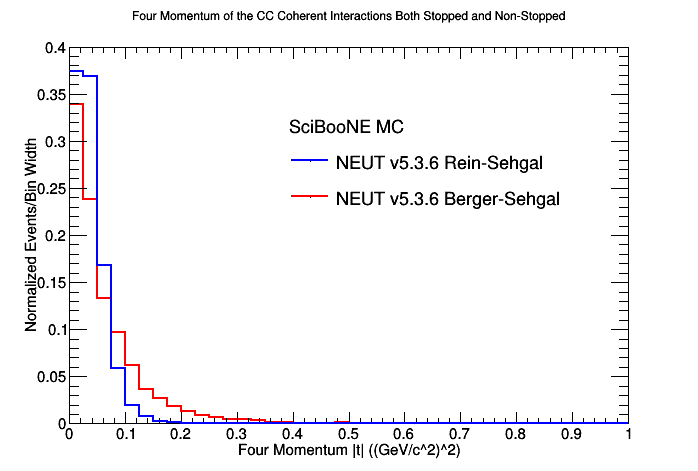
\includegraphics[width=0.4\textwidth]{CCCohPlots/ANMCCCohGoodT.png}
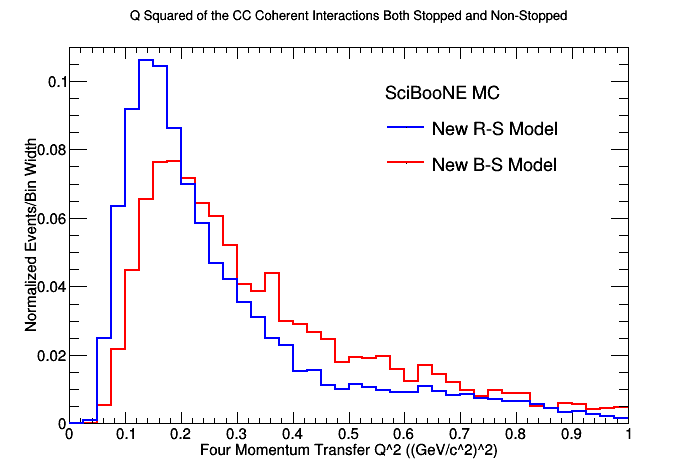
\includegraphics[width=0.4\textwidth]{CCCohPlots/ANMCCCohGoodQ2.png}
\caption{The $|t|$ Good Momentum Transfer (left) and $Q^2$ Good Momentum Transfer (right) for $\bar{\nu}$-mode CC-Coh $\pi^{+/-}$ interactions for both of the models included in this study. The Good classification means that this includes both the stopped and the not-stopped classifications of the CC-Coh $\pi^{+/-}$ events only.}
\end{figure}\label{fig:AntiNuModeCCCohGoodTAndQ2}
% This is where the t and q2 plots end


%=========================================================================
%=========================================================================
%
%=========================================================================
%=========================================================================
\newpage

\appendix


%=========================================================================
\section{Appendix: Sample Details}\label{sec:SampleAppendix}
%=========================================================================

Appendix on samples

%-----------------------------------------------------------------------------------------------------------------|
\subsection{$\nu$-Mode Rein-Sehgal NEUTv5.3.6}
A sample of 1,000,000 $\nu$ interactions were simulated using the NEUT generator (v5.3.6) and the Rein-Sehgal model for coherent pion production. This sample correspond to the file labeled 
\begin{verbatim}
SciBooNE_numu_coh_RooTrack.root
\end{verbatim}
found at the following link (put link to sample here).

%-----------------------------------------------------------------------------------------------------------------|
\subsection{$\nu$-Mode Berger-Sehgal NEUTv5.3.6}
A sample of 1,000,000 $\nu$ interactions were simulated using the NEUT generator (v5.3.6) and the Berger-Sehgal model for coherent pion production. This sample correspond to the file labeled
\begin{verbatim}
SciBooNE_numu_coh_RooTrack_NEW.root
\end{verbatim}
found at the following link (put link to sample here).



%-----------------------------------------------------------------------------------------------------------------|
\subsection{$\nu$-Mode Rein-Sehgal NEUTvx.x.x}
A sample of 100,000 $\nu$ interactions were simulated using the NEUT generator (vx.x.x, believed to be the version used by the SciBooNE collaboration in the original publication) and the corresponding older Rein-Sehgal model for coherent pion production. This sample correspond to the file labeled
\begin{verbatim}
SciBooNE_numu_coh_OLDNEUT_RooTrack.root
\end{verbatim}
found at the following link (put link to sample here).


%-----------------------------------------------------------------------------------------------------------------|
\subsection{$\bar{\nu}$-Mode Rein-Sehgal NEUTv5.3.6}
A sample of 1,000,000 $\bar{\nu}$ interactions were simulated using the NEUT generator (v5.3.6) and the Rein-Sehgal model for coherent pion production. This sample correspond to the file labeled
\begin{verbatim}
SciBooNE_numubar_coh_RooTrack.root
\end{verbatim}
found at the following link (put link to sample here).

%-----------------------------------------------------------------------------------------------------------------|
\subsection{$\bar{\nu}$-Mode Berger-Sehgal NEUTv5.3.6}
A sample of 1,000,000 $\bar{\nu}$ interactions were simulated using the NEUT generator (v5.3.6) and the Berger-Sehgal model for coherent pion production. This sample correspond to the file labeled
\begin{verbatim}
SciBooNE_numubar_coh_RooTrack_NEW.root
\end{verbatim}
found at the following link (put link to sample here).




%-----------------------------------------------------------------------------------------------------------------|
\subsection{Vertex Distributions}
The events were all given a random initial point that was generated with the goal that the vertex distributions of this simulation would closely match the vertex distributions that Hiraide (need to put a reference) showed in his thesis. This was done by... etc.

\begin{lstlisting}[language=C]
Put in the code for how we made the vertex distributions of the interactions.
\end{lstlisting}

\begin{figure}[H]
\centering
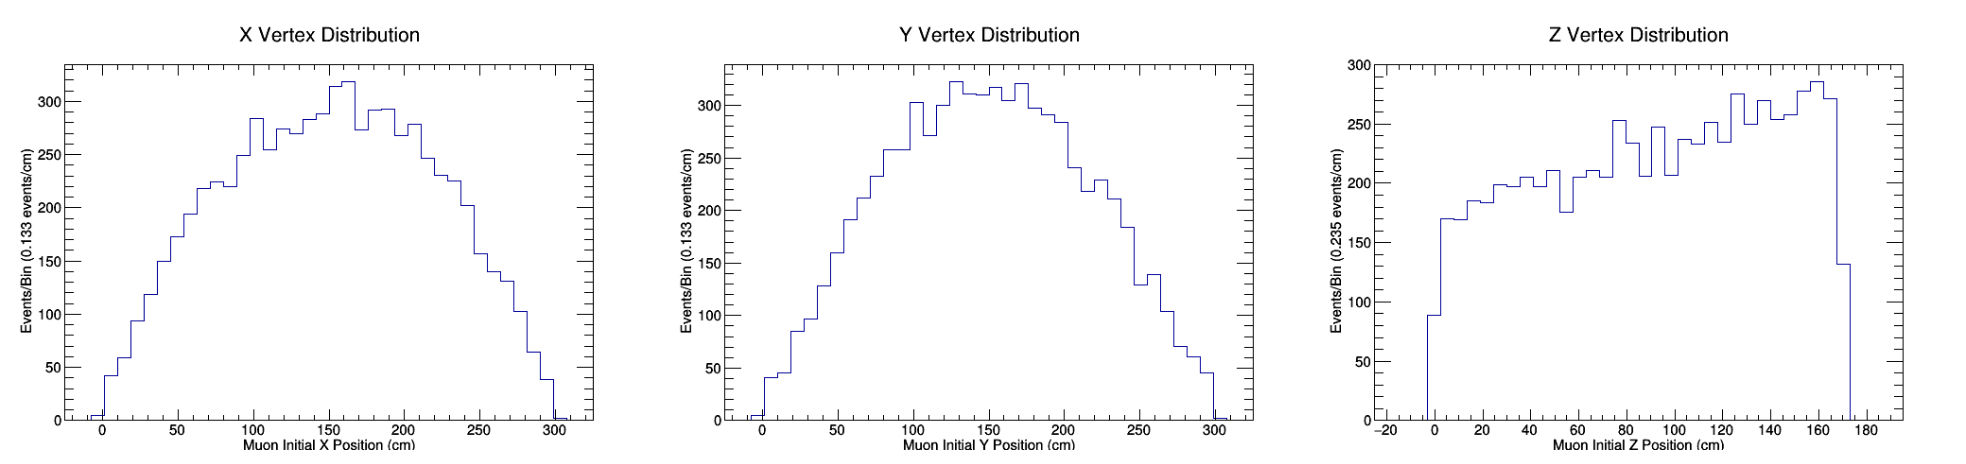
\includegraphics[width=1.0\textwidth]{EventClassifications/VertexDistributions.png}
\caption{Vertex distributions of the events in the new Rein-Sehgal sample.}
\end{figure}






%-----------------------------------------------------------------------------------------------------------------|
\subsection{NewNMReinSehgal.C}
This file is the macro that corresponds to the "NewNMReinSehgal.h" file, which connects with this file: "SciBooNE\textunderscore numu\textunderscore coh\textunderscore RooTrack.root". This file performs the main analysis for this generated sample, and then organizes the information into many different histograms. The histograms are then written to a file titled "totalmuoninfoRS.root" inside the "ROOTFILES" directory. The "ROOTFILES" directory is included in the SciBooNE-MC repository (it is absolutely pertinent that this directory be located where the macro files are located due to how the calls of the combined data macros reference the now saved histograms). When this macro is run (which can take a while), it also plots a few different histograms. The histograms that are plotted are the ones shown in the figures below with descriptions included with the corresponding figures. The order that the histograms appear in this paper is the same order they will be shown when this macro is run in root.

\begin{figure}[H]
\centering
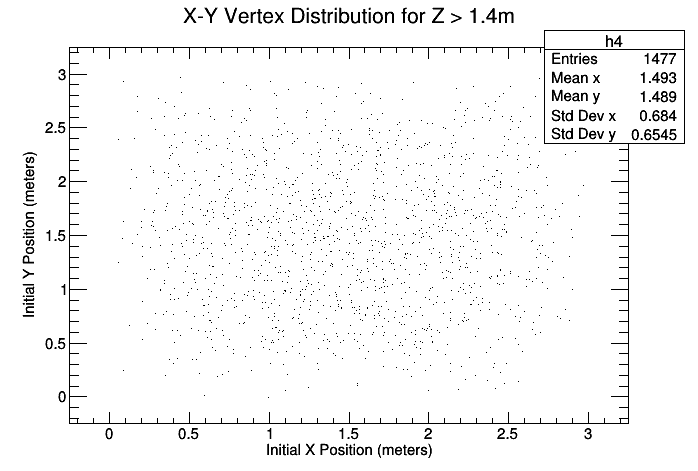
\includegraphics[width=0.6\textwidth]{NewNMReinSehgalImages/1-X-YVertexDistributionNMRS.png}
\caption{New $\nu$-Mode Rein-Sehgal X-Y vertex distributions for muons that made it to the MRD and penetrated at least to the third layer of steel.}
\end{figure}

\begin{figure}[H]
\centering
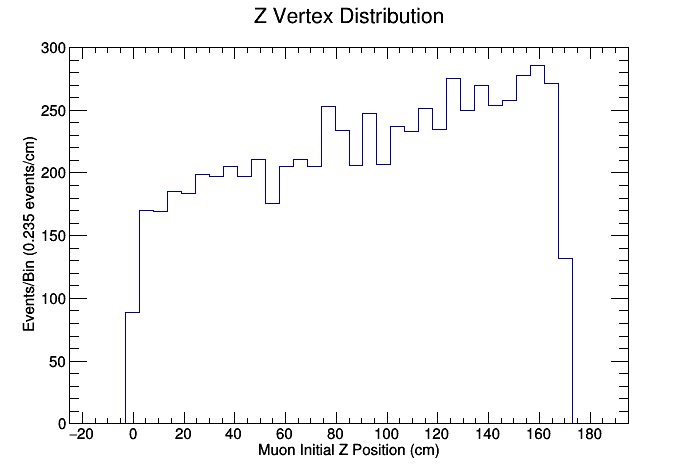
\includegraphics[width=0.6\textwidth]{NewNMReinSehgalImages/2-ZVertexDistributionNMRS.png}
\caption{New $\nu$-Mode Rein-Sehgal Z vertex distributions for the interactions.}
\end{figure}

\begin{figure}[H]
\centering
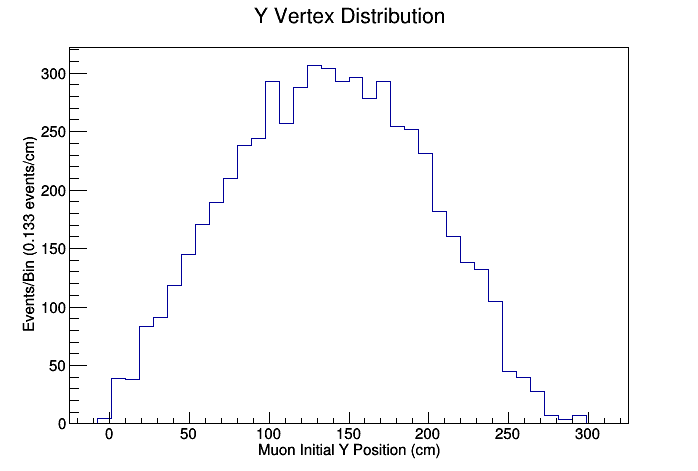
\includegraphics[width=0.6\textwidth]{NewNMReinSehgalImages/3-YVertexDistributionNMRS.png}
\caption{New $\nu$-Mode Rein-Sehgal Y vertex distributions for the interactions.}
\end{figure}

\begin{figure}[H]
\centering
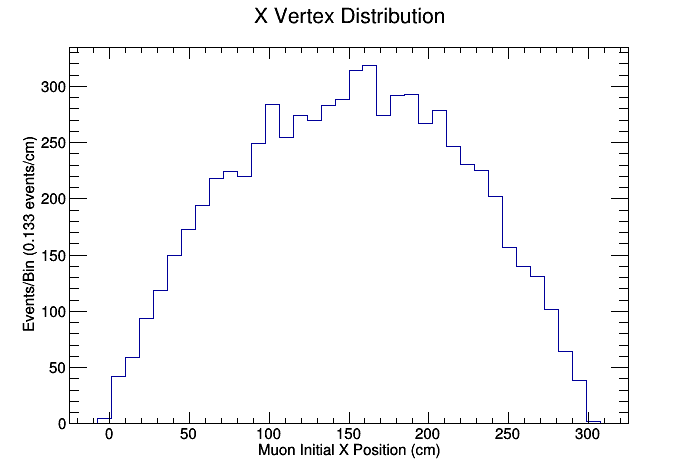
\includegraphics[width=0.6\textwidth]{NewNMReinSehgalImages/4-XVertexDistributionNMRS.png}
\caption{New $\nu$-Mode Rein-Sehgal X vertex distributions for the interactions.}
\end{figure}

\begin{figure}[H]
\centering
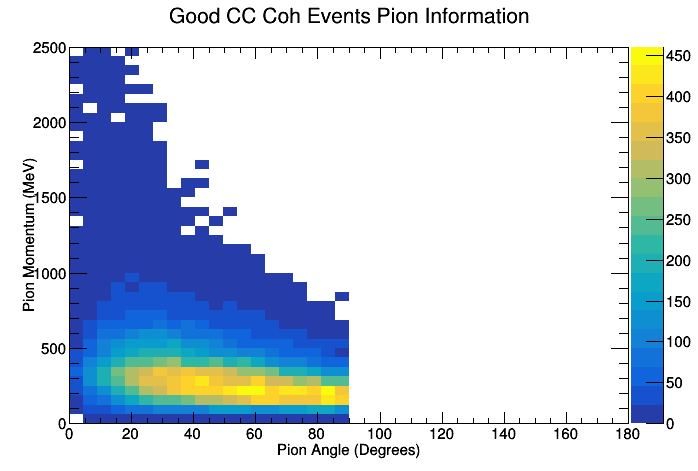
\includegraphics[width=0.6\textwidth]{NewNMReinSehgalImages/5-GoodCCCohPionInfoNMRS.png}
\caption{This is a 2D histogram for the momentum and angle of the pion in the CC Coh Pion events that met the qualification of being "good".}
\end{figure}

\begin{figure}[H]
\centering
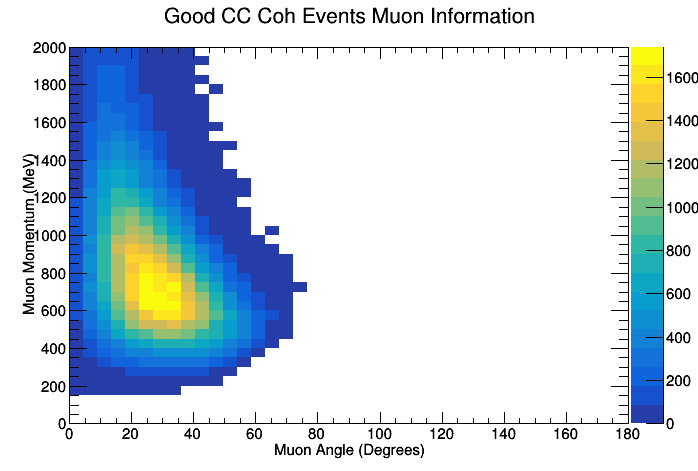
\includegraphics[width=0.6\textwidth]{NewNMReinSehgalImages/6-GoodCCCohMuonInfoNMRS.png}
\caption{This is a 2D histogram for the momentum and angle of the muon in the CC Coh Pion events that met the qualification of being "good".}
\end{figure}

\begin{figure}[H]
\centering
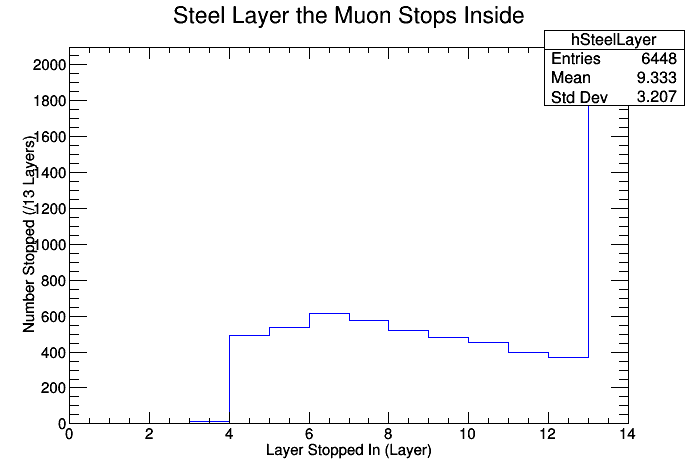
\includegraphics[width=0.6\textwidth]{NewNMReinSehgalImages/7-LayerPenetrationNMRS.png}
\caption{This histogram shows the amount of muons that embedded (or "Stopped") in a corresponding layer of steel in our simulation.}
\end{figure}

\begin{figure}[H]
\centering
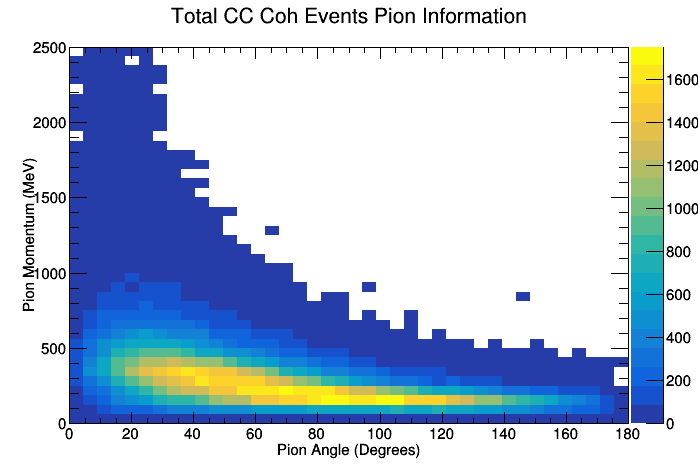
\includegraphics[width=0.6\textwidth]{NewNMReinSehgalImages/8-TotalCCCohPionInfoNMRS.png}
\caption{This is a 2D histogram for the momentum and angle of the pion in the total CC Coh Pion events.}
\end{figure}

\begin{figure}[H]
\centering
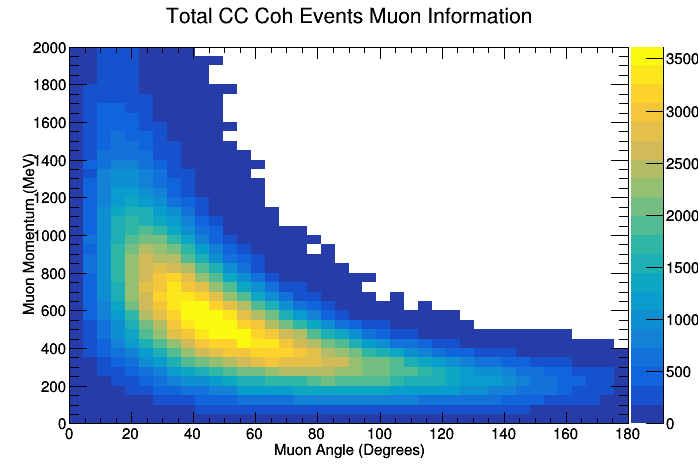
\includegraphics[width=0.6\textwidth]{NewNMReinSehgalImages/9-TotalCCCohMuonInfoNMRS.png}
\caption{This is a 2D histogram for the momentum and angle of the muon in the total CC Coh Pion events.}
\end{figure}

The NewNMReinSehgal.C macro also calculates many different quantities for the generated simulation of the events and saves the information in histograms that are later called upon through the plotting macros (which are after all of the analysis macros). The first quantity that is calculated for the different vertexes is the momentum of both the muon and the pion, which are both calculated using the equations:

\begin{equation}
|\vec{p}_\mu| = \sqrt{P_{\mu_x}^2 + P_{\mu_y}^2 + P_{\mu_z}^2}
\end{equation}

\begin{equation}
|\vec{p}_\pi| = \sqrt{P_{\pi_x}^2 + P_{\pi_y}^2 + P_{\pi_z}^2}
\end{equation}

\noindent
The momentum is reported in units of $MeV/c$.

The next quantity that is calculated in the macro is the angle from the beam-direction for both the muon and the pion, which are labeled as either $\theta_\mu$, or $\theta_\pi$, respectively. The angle from the beam-direction is the same as the angle from the z-direction, and this angle is known as the azimuthal angle. The calculation of the azimuthal angle is slightly more involved than the simple calculation used for finding the magnitude of the momentum of the two particles, and is calculated using the equations:

\begin{equation}
\theta_\mu = tan^{-1}(\sqrt{P_{\mu_x}^2 + P_{\mu_y}^2}/{P_{\mu_z}})
\end{equation}

\begin{equation}
\theta_\pi = tan^{-1}(\sqrt{P_{\pi_x}^2 + P_{\pi_y}^2}/{P_{\pi_z}})
\end{equation}

\noindent
The angles are reported in units of $\degree$, and should run from $0\degree$ to $180\degree$. In the case of Charged-Current Coherent Pion Production, the angle should never be larger than $90\degree$.

The last two quantities that this analysis macro calculates are the two different types of four-momentum transfers specific to this interaction, which are $Q^2$ and $|t|$. The $Q^2$ corresponds to the four-momentum transfer from the neutrino and muon to the nucleus and pion, and is calculated using the equation:

\begin{equation}
Q^2 = |(P_{\nu_\mu} - P_\mu)^2|
\end{equation}

\noindent
This equation is the four-momentum notational form. The code follows the equation below in order to compute $Q^2$:

\begin{equation}
Q^2 = |(P_{\nu_{\mu,x}} - P_{\mu_x})^2 + (P_{\nu_{\mu,y}} - P_{\mu_y})^2 + (P_{\nu_{\mu,z}} - P_{\mu_z})^2 + (P_{\nu_{\mu,E}} - P_{\mu_E})^2|
\end{equation}

\noindent
$Q^2$ is reported in units of $(MeV/c)^2$.

The $|t|$ corresponds to the four-momentum transfer from the neutrino, muon, and pion to the nucleus, and is calculated using the equation:

\begin{equation}
|t| = |(Q - P_\pi)^2| = |(P_{\nu_\mu} - P_\mu - P_\pi)^2|
\end{equation}

\noindent
This equation is the four-momentum notational form. The code follows the equation below in order to compute $|t|$:

\begin{equation}
|t| = |(P_{\nu_{\mu,x}} - P_{\mu_x} - P_{\pi_x})^2 + (P_{\nu_{\mu,y}} - P_{\mu_y} - P_{\pi_y})^2 + (P_{\nu_{\mu,z}} - P_{\mu_z} - P_{\pi_z})^2 + (P_{\nu_{\mu,E}} - P_{\mu_E} - P_{\pi_E})^2|
\end{equation}

\noindent
$|t|$ is reported in units of $(MeV/c)^2$.

%-----------------------------------------------------------------------------------------------------------------|
\subsection{NewNMBergerSehgal.C}
This file is the macro that corresponds to the "NewNMBergerSehgal.h" file, which connects with this file: "SciBooNE\textunderscore numu\textunderscore coh\textunderscore RooTrack\textunderscore NEW.root". This file performs the main analysis for this generated sample, and then organizes the information into many different histograms. The histograms are then written to a file titled "totalmuoninfoBS.root" inside the "ROOTFILES" directory. The "ROOTFILES" directory is included in the SciBooNE-MC repository (it is absolutely pertinent that this directory be located where the macro files are located due to how the calls of the combined data macros reference the now saved histograms).

\begin{figure}[H]
\centering
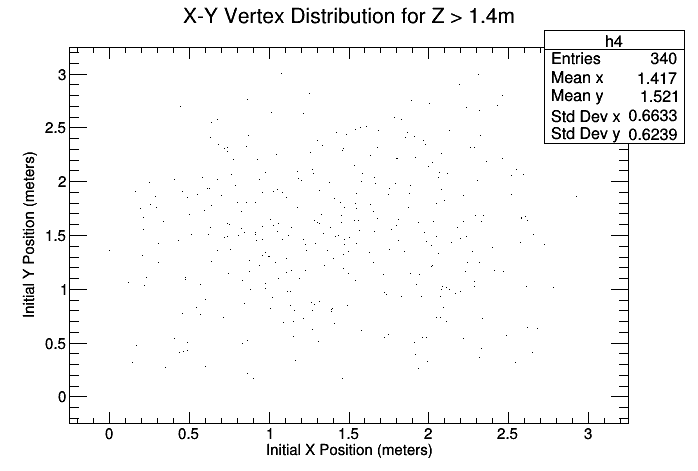
\includegraphics[width=0.6\textwidth]{NewNMBergerSehgalImages/1-X-YVertexDistributionNMBS.png}
\caption{New $\nu$-Mode Berger-Sehgal X-Y vertex distributions for muons that made it to the MRD and penetrated at least to the third layer of steel.}
\end{figure}

\begin{figure}[H]
\centering
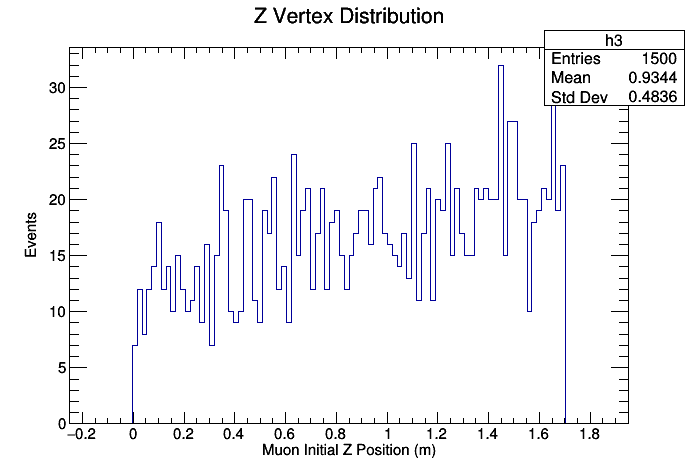
\includegraphics[width=0.6\textwidth]{NewNMBergerSehgalImages/2-ZVertexDistributionNMBS.png}
\caption{New $\nu$-Mode Berger-Sehgal Z vertex distributions for the interactions.}
\end{figure}

\begin{figure}[H]
\centering
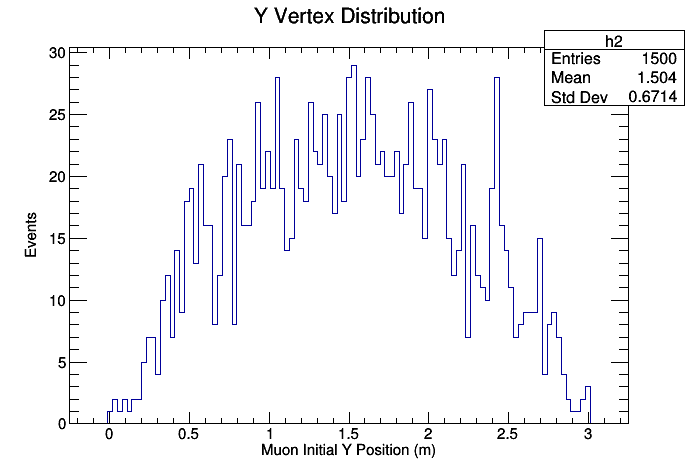
\includegraphics[width=0.6\textwidth]{NewNMBergerSehgalImages/3-YVertexDistributionNMBS.png}
\caption{New $\nu$-Mode Berger-Sehgal Y vertex distributions for the interactions.}
\end{figure}

\begin{figure}[H]
\centering
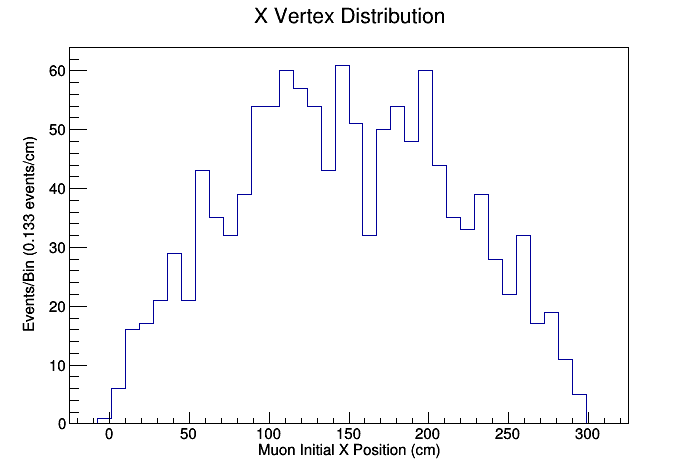
\includegraphics[width=0.6\textwidth]{NewNMBergerSehgalImages/4-XVertexDistributionNMBS.png}
\caption{New $\nu$-Mode Berger-Sehgal X vertex distributions for the interactions.}
\end{figure}

\begin{figure}[H]
\centering
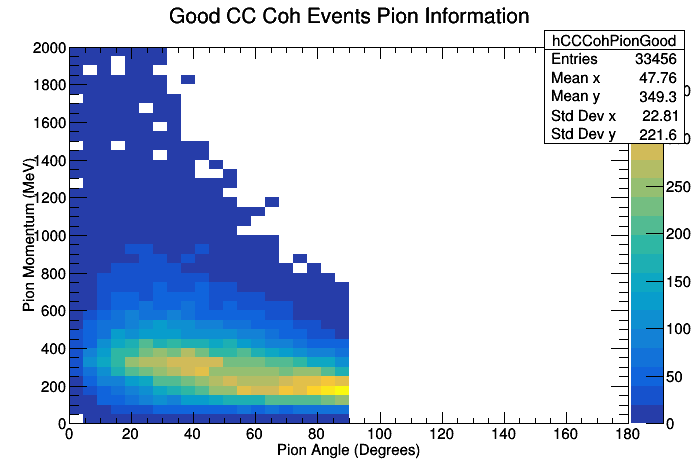
\includegraphics[width=0.6\textwidth]{NewNMBergerSehgalImages/5-GoodCCCohPionInfoNMBS.png}
\caption{This is a 2D histogram for the momentum and angle of the pion in the CC Coh Pion events that met the qualification of being "good".}
\end{figure}

\begin{figure}[H]
\centering
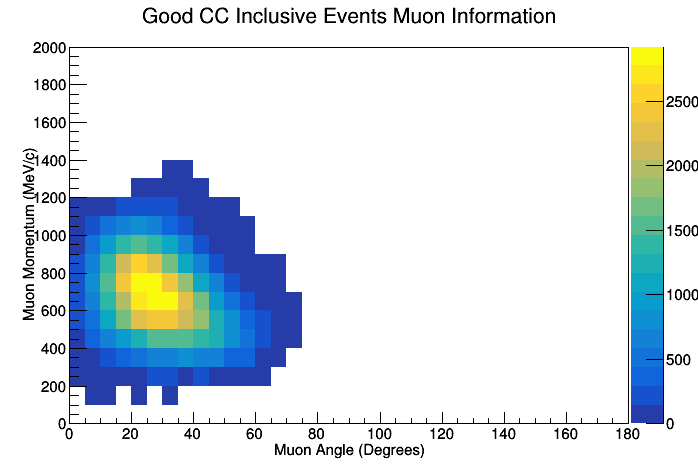
\includegraphics[width=0.6\textwidth]{NewNMBergerSehgalImages/6-GoodCCCohMuonInfoNMBS.png}
\caption{This is a 2D histogram for the momentum and angle of the muon in the CC Coh Pion events that met the qualification of being "good".!}
\end{figure}

\begin{figure}[H]
\centering
\includegraphics[width=0.6\textwidth]{NewNMBergerSehgalImages/7-LayerPenetrationNMBS.png}
\caption{This histogram shows the amount of muons that embedded (or "Stopped") in a corresponding layer of steel in our simulation.}
\end{figure}

\begin{figure}[H]
\centering
\includegraphics[width=0.6\textwidth]{NewNMBergerSehgalImages/8-TotalCCCohPionInfoNMBS.png}
\caption{This is a 2D histogram for the momentum and angle of the pion in the total CC Coh Pion events.}
\end{figure}

\begin{figure}[H]
\centering
\includegraphics[width=0.6\textwidth]{NewNMBergerSehgalImages/9-TotalCCCohMuonInfoNMBS.png}
\caption{This is a 2D histogram for the momentum and angle of the muon in the total CC Coh Pion events.}
\end{figure}

The NewNMBergerSehgal.C macro also calculates many different quantities for the generated simulation of the events and saves the information in histograms that are later called upon through the plotting macros (which are after all of the analysis macros). The first quantity that is calculated for the different vertexes is the momentum of both the muon and the pion, which are both calculated using the equations:

\begin{equation}
|\vec{p}_\mu| = \sqrt{P_{\mu_x}^2 + P_{\mu_y}^2 + P_{\mu_z}^2}
\end{equation}

\begin{equation}
|\vec{p}_\pi| = \sqrt{P_{\pi_x}^2 + P_{\pi_y}^2 + P_{\pi_z}^2}
\end{equation}

\noindent
The momentum is reported in units of $MeV/c$.

The next quantity that is calculated in the macro is the angle from the beam-direction for both the muon and the pion, which are labeled as either $\theta_\mu$, or $\theta_\pi$, respectively. The angle from the beam-direction is the same as the angle from the z-direction, and this angle is known as the azimuthal angle. The calculation of the azimuthal angle is slightly more involved than the simple calculation used for finding the magnitude of the momentum of the two particles, and is calculated using the equations:

\begin{equation}
\theta_\mu = tan^{-1}(\sqrt{P_{\mu_x}^2 + P_{\mu_y}^2}/{P_{\mu_z}})
\end{equation}

\begin{equation}
\theta_\pi = tan^{-1}(\sqrt{P_{\pi_x}^2 + P_{\pi_y}^2}/{P_{\pi_z}})
\end{equation}

\noindent
The angles are reported in units of $\degree$, and should run from $0\degree$ to $180\degree$. In the case of Charged-Current Coherent Pion Production, the angle should never be larger than $90\degree$.

The last two quantities that this analysis macro calculates are the two different types of four-momentum transfers specific to this interaction, which are $Q^2$ and $|t|$. The $Q^2$ corresponds to the four-momentum transfer from the neutrino and muon to the nucleus and pion, and is calculated using the equation:

\begin{equation}
Q^2 = |(P_{\nu_\mu} - P_\mu)^2|
\end{equation}

\noindent
This equation is the four-momentum notational form. The code follows the equation below in order to compute $Q^2$:

\begin{equation}
Q^2 = |(P_{\nu_{\mu,x}} - P_{\mu_x})^2 + (P_{\nu_{\mu,y}} - P_{\mu_y})^2 + (P_{\nu_{\mu,z}} - P_{\mu_z})^2 + (P_{\nu_{\mu,E}} - P_{\mu_E})^2|
\end{equation}

\noindent
$Q^2$ is reported in units of $(MeV/c)^2$.

The $|t|$ corresponds to the four-momentum transfer from the neutrino, muon, and pion to the nucleus, and is calculated using the equation:

\begin{equation}
|t| = |(Q - P_\pi)^2| = |(P_{\nu_\mu} - P_\mu - P_\pi)^2|
\end{equation}

\noindent
This equation is the four-momentum notational form. The code follows the equation below in order to compute $|t|$:

\begin{equation}
|t| = |(P_{\nu_{\mu,x}} - P_{\mu_x} - P_{\pi_x})^2 + (P_{\nu_{\mu,y}} - P_{\mu_y} - P_{\pi_y})^2 + (P_{\nu_{\mu,z}} - P_{\mu_z} - P_{\pi_z})^2 + (P_{\nu_{\mu,E}} - P_{\mu_E} - P_{\pi_E})^2|
\end{equation}

\noindent
$|t|$ is reported in units of $(MeV/c)^2$.

%-----------------------------------------------------------------------------------------------------------------|
\subsection{OldNMReinSehgal.C}
This file is the macro that corresponds to the "OldNMReinSehgal.h" file, which connects with this file: "SciBooNE\textunderscore numu\textunderscore coh\textunderscore OLDNEUT\textunderscore RooTrack.root". This file performs the main analysis for this generated sample, and then organizes the information into many different histograms. The histograms are then written to a file titled "totalmuoninfoOBS.root" inside the "ROOTFILES" directory. The "ROOTFILES" directory is included in the SciBooNE-MC repository (it is absolutely pertinent that this directory be located where the macro files are located due to how the calls of the combined data macros reference the now saved histograms).

\begin{figure}[H]
\centering
\includegraphics[width=0.6\textwidth]{OldNMReinSehgalImages/1-X-YVertexDistributionNMORS.png}
\caption{Old $\nu$-Mode Rein-Sehgal X-Y vertex distributions for muons that made it to the MRD and penetrated at least to the third layer of steel.}
\end{figure}

\begin{figure}[H]
\centering
\includegraphics[width=0.6\textwidth]{OldNMReinSehgalImages/2-ZVertexDistributionNMORS.png}
\caption{Old $\nu$-Mode Rein-Sehgal Z vertex distributions for the interactions.}
\end{figure}

\begin{figure}[H]
\centering
\includegraphics[width=0.6\textwidth]{OldNMReinSehgalImages/3-YVertexDistributionNMORS.png}
\caption{Old $\nu$-Mode Rein-Sehgal Y vertex distributions for the interactions.}
\end{figure}

\begin{figure}[H]
\centering
\includegraphics[width=0.6\textwidth]{OldNMReinSehgalImages/4-XVertexDistributionNMORS.png}
\caption{Old $\nu$-Mode Rein-Sehgal X vertex distributions for the interactions.}
\end{figure}

\begin{figure}[H]
\centering
\includegraphics[width=0.6\textwidth]{OldNMReinSehgalImages/5-GoodCCCohPionInfoNMORS.png}
\caption{This is a 2D histogram for the momentum and angle of the pion in the CC Coh Pion events that met the qualification of being "good".}
\end{figure}

\begin{figure}[H]
\centering
\includegraphics[width=0.6\textwidth]{OldNMReinSehgalImages/6-GoodCCCohMuonInfoNMORS.png}
\caption{This is a 2D histogram for the momentum and angle of the muon in the CC Coh Pion events that met the qualification of being "good".}
\end{figure}

\begin{figure}[H]
\centering
\includegraphics[width=0.6\textwidth]{OldNMReinSehgalImages/7-LayerPenetrationNMORS.png}
\caption{This histogram shows the amount of muons that embedded (or "Stopped") in a corresponding layer of steel in our simulation.}
\end{figure}

\begin{figure}[H]
\centering
\includegraphics[width=0.6\textwidth]{OldNMReinSehgalImages/8-TotalCCCohPionInfoNMORS.png}
\caption{This is a 2D histogram for the momentum and angle of the pion in the total CC Coh Pion events.}
\end{figure}

\begin{figure}[H]
\centering
\includegraphics[width=0.6\textwidth]{OldNMReinSehgalImages/9-TotalCCCohMuonInfoNMORS.png}
\caption{This is a 2D histogram for the momentum and angle of the muon in the total CC Coh Pion events.}
\end{figure}

The OldNMReinSehgal.C macro also calculates many different quantities for the generated simulation of the events and saves the information in histograms that are later called upon through the plotting macros (which are after all of the analysis macros). The first quantity that is calculated for the different vertexes is the momentum of both the muon and the pion, which are both calculated using the equations:

\begin{equation}
|\vec{p}_\mu| = \sqrt{P_{\mu_x}^2 + P_{\mu_y}^2 + P_{\mu_z}^2}
\end{equation}

\begin{equation}
|\vec{p}_\pi| = \sqrt{P_{\pi_x}^2 + P_{\pi_y}^2 + P_{\pi_z}^2}
\end{equation}

\noindent
The momentum is reported in units of $MeV/c$.

The next quantity that is calculated in the macro is the angle from the beam-direction for both the muon and the pion, which are labeled as either $\theta_\mu$, or $\theta_\pi$, respectively. The angle from the beam-direction is the same as the angle from the z-direction, and this angle is known as the azimuthal angle. The calculation of the azimuthal angle is slightly more involved than the simple calculation used for finding the magnitude of the momentum of the two particles, and is calculated using the equations:

\begin{equation}
\theta_\mu = tan^{-1}(\sqrt{P_{\mu_x}^2 + P_{\mu_y}^2}/{P_{\mu_z}})
\end{equation}

\begin{equation}
\theta_\pi = tan^{-1}(\sqrt{P_{\pi_x}^2 + P_{\pi_y}^2}/{P_{\pi_z}})
\end{equation}

\noindent
The angles are reported in units of $\degree$, and should run from $0\degree$ to $180\degree$. In the case of Charged-Current Coherent Pion Production, the angle should never be larger than $90\degree$.

The last two quantities that this analysis macro calculates are the two different types of four-momentum transfers specific to this interaction, which are $Q^2$ and $|t|$. The $Q^2$ corresponds to the four-momentum transfer from the neutrino and muon to the nucleus and pion, and is calculated using the equation:

\begin{equation}
Q^2 = |(P_{\nu_\mu} - P_\mu)^2|
\end{equation}

\noindent
This equation is the four-momentum notational form. The code follows the equation below in order to compute $Q^2$:

\begin{equation}
Q^2 = |(P_{\nu_{\mu,x}} - P_{\mu_x})^2 + (P_{\nu_{\mu,y}} - P_{\mu_y})^2 + (P_{\nu_{\mu,z}} - P_{\mu_z})^2 + (P_{\nu_{\mu,E}} - P_{\mu_E})^2|
\end{equation}

\noindent
$Q^2$ is reported in units of $(MeV/c)^2$.

The $|t|$ corresponds to the four-momentum transfer from the neutrino, muon, and pion to the nucleus, and is calculated using the equation:

\begin{equation}
|t| = |(Q - P_\pi)^2| = |(P_{\nu_\mu} - P_\mu - P_\pi)^2|
\end{equation}

\noindent
This equation is the four-momentum notational form. The code follows the equation below in order to compute $|t|$:

\begin{equation}
|t| = |(P_{\nu_{\mu,x}} - P_{\mu_x} - P_{\pi_x})^2 + (P_{\nu_{\mu,y}} - P_{\mu_y} - P_{\pi_y})^2 + (P_{\nu_{\mu,z}} - P_{\mu_z} - P_{\pi_z})^2 + (P_{\nu_{\mu,E}} - P_{\mu_E} - P_{\pi_E})^2|
\end{equation}

\noindent
$|t|$ is reported in units of $(MeV/c)^2$.

%-----------------------------------------------------------------------------------------------------------------|
\subsection{NewANMReinSehgal.C}
This file is the macro that corresponds to the "NewANMReinSehgal.h" file, which connects with this file: "SciBooNE\textunderscore numubar\textunderscore coh\textunderscore RooTrack.root". This file performs the main analysis for this generated sample, and then organizes the information into many different histograms. The histograms are then written to a file titled "totalmuoninfoRSBar.root" inside the "ROOTFILES" directory. The "ROOTFILES" directory is included in the SciBooNE-MC repository (it is absolutely pertinent that this directory be located where the macro files are located due to how the calls of the combined data macros reference the now saved histograms).

\begin{figure}[H]
\centering
\includegraphics[width=0.6\textwidth]{NewANMReinSehgalImages/1-X-YVertexDistributionANMRS.png}
\caption{New $\bar{\nu}$-Mode Rein-Sehgal X-Y vertex distributions for muons that made it to the MRD and penetrated at least to the third layer of steel.}
\end{figure}

\begin{figure}[H]
\centering
\includegraphics[width=0.6\textwidth]{NewANMReinSehgalImages/2-ZVertexDistributionANMRS.png}
\caption{New $\bar{\nu}$-Mode Rein-Sehgal Z vertex distributions for the interactions.}
\end{figure}

\begin{figure}[H]
\centering
\includegraphics[width=0.6\textwidth]{NewANMReinSehgalImages/3-YVertexDistributionANMRS.png}
\caption{New $\bar{\nu}$-Mode Rein-Sehgal Y vertex distributions for the interactions.}
\end{figure}

\begin{figure}[H]
\centering
\includegraphics[width=0.6\textwidth]{NewANMReinSehgalImages/4-XVertexDistributionANMRS.png}
\caption{New $\bar{\nu}$-Mode Rein-Sehgal X vertex distributions for the interactions.}
\end{figure}

\begin{figure}[H]
\centering
\includegraphics[width=0.6\textwidth]{NewANMReinSehgalImages/5-GoodCCCohPionInfoANMRS.png}
\caption{This is a 2D histogram for the momentum and angle of the pion in the CC Coh Pion events that met the qualification of being "good".}
\end{figure}

\begin{figure}[H]
\centering
\includegraphics[width=0.6\textwidth]{NewANMReinSehgalImages/6-GoodCCCohMuonInfoANMRS.png}
\caption{This is a 2D histogram for the momentum and angle of the muon in the CC Coh Pion events that met the qualification of being "good".}
\end{figure}

\begin{figure}[H]
\centering
\includegraphics[width=0.6\textwidth]{NewANMReinSehgalImages/7-LayerPenetrationANMRS.png}
\caption{This histogram shows the amount of muons that embedded (or "Stopped") in a corresponding layer of steel in our simulation.}
\end{figure}

\begin{figure}[H]
\centering
\includegraphics[width=0.6\textwidth]{NewANMReinSehgalImages/8-TotalCCCohPionInfoANMRS.png}
\caption{This is a 2D histogram for the momentum and angle of the pion in the total CC Coh Pion events.}
\end{figure}

\begin{figure}[H]
\centering
\includegraphics[width=0.6\textwidth]{NewANMReinSehgalImages/9-TotalCCCohMuonInfoANMRS.png}
\caption{This is a 2D histogram for the momentum and angle of the muon in the total CC Coh Pion events.}
\end{figure}

The NewANMReinSehgal.C macro also calculates many different quantities for the generated simulation of the events and saves the information in histograms that are later called upon through the plotting macros (which are after all of the analysis macros). The first quantity that is calculated for the different vertexes is the momentum of both the muon and the pion, which are both calculated using the equations:

\begin{equation}
|\vec{p}_\mu| = \sqrt{P_{\mu_x}^2 + P_{\mu_y}^2 + P_{\mu_z}^2}
\end{equation}

\begin{equation}
|\vec{p}_\pi| = \sqrt{P_{\pi_x}^2 + P_{\pi_y}^2 + P_{\pi_z}^2}
\end{equation}

\noindent
The momentum is reported in units of $MeV/c$.

The next quantity that is calculated in the macro is the angle from the beam-direction for both the muon and the pion, which are labeled as either $\theta_\mu$, or $\theta_\pi$, respectively. The angle from the beam-direction is the same as the angle from the z-direction, and this angle is known as the azimuthal angle. The calculation of the azimuthal angle is slightly more involved than the simple calculation used for finding the magnitude of the momentum of the two particles, and is calculated using the equations:

\begin{equation}
\theta_\mu = tan^{-1}(\sqrt{P_{\mu_x}^2 + P_{\mu_y}^2}/{P_{\mu_z}})
\end{equation}

\begin{equation}
\theta_\pi = tan^{-1}(\sqrt{P_{\pi_x}^2 + P_{\pi_y}^2}/{P_{\pi_z}})
\end{equation}

\noindent
The angles are reported in units of $\degree$, and should run from $0\degree$ to $180\degree$. In the case of Charged-Current Coherent Pion Production, the angle should never be larger than $90\degree$.

The last two quantities that this analysis macro calculates are the two different types of four-momentum transfers specific to this interaction, which are $Q^2$ and $|t|$. The $Q^2$ corresponds to the four-momentum transfer from the neutrino and muon to the nucleus and pion, and is calculated using the equation:

\begin{equation}
Q^2 = |(P_{\nu_\mu} - P_\mu)^2|
\end{equation}

\noindent
This equation is the four-momentum notational form. The code follows the equation below in order to compute $Q^2$:

\begin{equation}
Q^2 = |(P_{\nu_{\mu,x}} - P_{\mu_x})^2 + (P_{\nu_{\mu,y}} - P_{\mu_y})^2 + (P_{\nu_{\mu,z}} - P_{\mu_z})^2 + (P_{\nu_{\mu,E}} - P_{\mu_E})^2|
\end{equation}

\noindent
$Q^2$ is reported in units of $(MeV/c)^2$.

The $|t|$ corresponds to the four-momentum transfer from the neutrino, muon, and pion to the nucleus, and is calculated using the equation:

\begin{equation}
|t| = |(Q - P_\pi)^2| = |(P_{\nu_\mu} - P_\mu - P_\pi)^2|
\end{equation}

\noindent
This equation is the four-momentum notational form. The code follows the equation below in order to compute $|t|$:

\begin{equation}
|t| = |(P_{\nu_{\mu,x}} - P_{\mu_x} - P_{\pi_x})^2 + (P_{\nu_{\mu,y}} - P_{\mu_y} - P_{\pi_y})^2 + (P_{\nu_{\mu,z}} - P_{\mu_z} - P_{\pi_z})^2 + (P_{\nu_{\mu,E}} - P_{\mu_E} - P_{\pi_E})^2|
\end{equation}

\noindent
$|t|$ is reported in units of $(MeV/c)^2$.

%-----------------------------------------------------------------------------------------------------------------|
\subsection{NewANMBergerSehgal.C}
This file is the macro that corresponds to the "NewANMBergerSehgal.h" file, which connects with this file: "SciBooNE\textunderscore numubar\textunderscore coh\textunderscore RooTrack\textunderscore NEW.root". This file performs the main analysis for this generated sample, and then organizes the information into many different histograms. The histograms are then written to a file titled "totalmuoninfoBSBar.root" inside the "ROOTFILES" directory. The "ROOTFILES" directory is included in the SciBooNE-MC repository (it is absolutely pertinent that this directory be located where the macro files are located due to how the calls of the combined data macros reference the now saved histograms).

\begin{figure}[H]
\centering
\includegraphics[width=0.6\textwidth]{NewANMBergerSehgalImages/1-X-YVertexDistributionANMBS.png}
\caption{New $\bar{\nu}$-Mode Berger-Sehgal X-Y vertex distributions for muons that made it to the MRD and penetrated at least to the third layer of steel.}
\end{figure}

\begin{figure}[H]
\centering
\includegraphics[width=0.6\textwidth]{NewANMBergerSehgalImages/2-ZVertexDistributionANMBS.png}
\caption{New $\bar{\nu}$-Mode Berger-Sehgal Z vertex distributions for the interactions.}
\end{figure}

\begin{figure}[H]
\centering
\includegraphics[width=0.6\textwidth]{NewANMBergerSehgalImages/3-YVertexDistributionANMBS.png}
\caption{New $\bar{\nu}$-Mode Berger-Sehgal Y vertex distributions for the interactions.}
\end{figure}

\begin{figure}[H]
\centering
\includegraphics[width=0.6\textwidth]{NewANMBergerSehgalImages/4-XVertexDistributionANMBS.png}
\caption{New $\bar{\nu}$-Mode Berger-Sehgal X vertex distributions for the interactions.}
\end{figure}

\begin{figure}[H]
\centering
\includegraphics[width=0.6\textwidth]{NewANMBergerSehgalImages/5-GoodCCCohPionInfoANMBS.png}
\caption{This is a 2D histogram for the momentum and angle of the pion in the CC Coh Pion events that met the qualification of being "good".}
\end{figure}

\begin{figure}[H]
\centering
\includegraphics[width=0.6\textwidth]{NewANMBergerSehgalImages/6-GoodCCCohMuonInfoANMBS.png}
\caption{This is a 2D histogram for the momentum and angle of the muon in the CC Coh Pion events that met the qualification of being "good".}
\end{figure}

\begin{figure}[H]
\centering
\includegraphics[width=0.6\textwidth]{NewANMBergerSehgalImages/7-LayerPenetrationANMBS.png}
\caption{This histogram shows the amount of muons that embedded (or "Stopped") in a corresponding layer of steel in our simulation.}
\end{figure}

\begin{figure}[H]
\centering
\includegraphics[width=0.6\textwidth]{NewANMBergerSehgalImages/8-TotalCCCohPionInfoANMBS.png}
\caption{This is a 2D histogram for the momentum and angle of the pion in the total CC Coh Pion events.}
\end{figure}

\begin{figure}[H]
\centering
\includegraphics[width=0.6\textwidth]{NewANMBergerSehgalImages/9-TotalCCCohMuonInfoANMBS.png}
\caption{This is a 2D histogram for the momentum and angle of the muon in the total CC Coh Pion events.}
\end{figure}

The NewANMBergerSehgal.C macro also calculates many different quantities for the generated simulation of the events and saves the information in histograms that are later called upon through the plotting macros (which are after all of the analysis macros). The first quantity that is calculated for the different vertexes is the momentum of both the muon and the pion, which are both calculated using the equations:

\begin{equation}
|\vec{p}_\mu| = \sqrt{P_{\mu_x}^2 + P_{\mu_y}^2 + P_{\mu_z}^2}
\end{equation}

\begin{equation}
|\vec{p}_\pi| = \sqrt{P_{\pi_x}^2 + P_{\pi_y}^2 + P_{\pi_z}^2}
\end{equation}

\noindent
The momentum is reported in units of $MeV/c$.

The next quantity that is calculated in the macro is the angle from the beam-direction for both the muon and the pion, which are labeled as either $\theta_\mu$, or $\theta_\pi$, respectively. The angle from the beam-direction is the same as the angle from the z-direction, and this angle is known as the azimuthal angle. The calculation of the azimuthal angle is slightly more involved than the simple calculation used for finding the magnitude of the momentum of the two particles, and is calculated using the equations:

\begin{equation}
\theta_\mu = tan^{-1}(\sqrt{P_{\mu_x}^2 + P_{\mu_y}^2}/{P_{\mu_z}})
\end{equation}

\begin{equation}
\theta_\pi = tan^{-1}(\sqrt{P_{\pi_x}^2 + P_{\pi_y}^2}/{P_{\pi_z}})
\end{equation}

\noindent
The angles are reported in units of $\degree$, and should run from $0\degree$ to $180\degree$. In the case of Charged-Current Coherent Pion Production, the angle should never be larger than $90\degree$.

The last two quantities that this analysis macro calculates are the two different types of four-momentum transfers specific to this interaction, which are $Q^2$ and $|t|$. The $Q^2$ corresponds to the four-momentum transfer from the neutrino and muon to the nucleus and pion, and is calculated using the equation:

\begin{equation}
Q^2 = |(P_{\nu_\mu} - P_\mu)^2|
\end{equation}

\noindent
This equation is the four-momentum notational form. The code follows the equation below in order to compute $Q^2$:

\begin{equation}
Q^2 = |(P_{\nu_{\mu,x}} - P_{\mu_x})^2 + (P_{\nu_{\mu,y}} - P_{\mu_y})^2 + (P_{\nu_{\mu,z}} - P_{\mu_z})^2 + (P_{\nu_{\mu,E}} - P_{\mu_E})^2|
\end{equation}

\noindent
$Q^2$ is reported in units of $(MeV/c)^2$.

The $|t|$ corresponds to the four-momentum transfer from the neutrino, muon, and pion to the nucleus, and is calculated using the equation:

\begin{equation}
|t| = |(Q - P_\pi)^2| = |(P_{\nu_\mu} - P_\mu - P_\pi)^2|
\end{equation}

\noindent
This equation is the four-momentum notational form. The code follows the equation below in order to compute $|t|$:

\begin{equation}
|t| = |(P_{\nu_{\mu,x}} - P_{\mu_x} - P_{\pi_x})^2 + (P_{\nu_{\mu,y}} - P_{\mu_y} - P_{\pi_y})^2 + (P_{\nu_{\mu,z}} - P_{\mu_z} - P_{\pi_z})^2 + (P_{\nu_{\mu,E}} - P_{\mu_E} - P_{\pi_E})^2|
\end{equation}

\noindent
$|t|$ is reported in units of $(MeV/c)^2$.

%-----------------------------------------------------------------------------------------------------------------|
\subsection{NMCombinedPlots.C}
I need to come back and insert all of my images here.

\begin{figure}[H]
\centering
\includegraphics[width=0.6\textwidth]{NMCombinedPlotsImages/1-NMCombinedPlots.png}
\caption{}
\end{figure}

\begin{figure}[H]
\centering
\includegraphics[width=0.6\textwidth]{NMCombinedPlotsImages/2-NMCombinedPlots.png}
\caption{}
\end{figure}

\begin{figure}[H]
\centering
\includegraphics[width=0.6\textwidth]{NMCombinedPlotsImages/3-NMCombinedPlots.png}
\caption{}
\end{figure}

\begin{figure}[H]
\centering
\includegraphics[width=0.6\textwidth]{NMCombinedPlotsImages/4-NMCombinedPlots.png}
\caption{}
\end{figure}

\begin{figure}[H]
\centering
\includegraphics[width=0.6\textwidth]{NMCombinedPlotsImages/5-NMCombinedPlots.png}
\caption{}
\end{figure}

\begin{figure}[H]
\centering
\includegraphics[width=0.6\textwidth]{NMCombinedPlotsImages/6-NMCombinedPlots.png}
\caption{}
\end{figure}

\begin{figure}[H]
\centering
\includegraphics[width=0.6\textwidth]{NMCombinedPlotsImages/7-NMCombinedPlots.png}
\caption{}
\end{figure}

\begin{figure}[H]
\centering
\includegraphics[width=0.6\textwidth]{NMCombinedPlotsImages/8-NMCombinedPlots.png}
\caption{}
\end{figure}

\begin{figure}[H]
\centering
\includegraphics[width=0.6\textwidth]{NMCombinedPlotsImages/9-NMCombinedPlots.png}
\caption{}
\end{figure}

\begin{figure}[H]
\centering
\includegraphics[width=0.6\textwidth]{NMCombinedPlotsImages/10-NMCombinedPlots.png}
\caption{}
\end{figure}

\begin{figure}[H]
\centering
\includegraphics[width=0.6\textwidth]{NMCombinedPlotsImages/11-NMCombinedPlots.png}
\caption{}
\end{figure}

\begin{figure}[H]
\centering
\includegraphics[width=0.6\textwidth]{NMCombinedPlotsImages/12-NMCombinedPlots.png}
\caption{}
\end{figure}

\begin{figure}[H]
\centering
\includegraphics[width=0.6\textwidth]{NMCombinedPlotsImages/13-NMCombinedPlots.png}
\caption{}
\end{figure}

\begin{figure}[H]
\centering
\includegraphics[width=0.6\textwidth]{NMCombinedPlotsImages/14-NMCombinedPlots.png}
\caption{}
\end{figure}

\begin{figure}[H]
\centering
\includegraphics[width=0.6\textwidth]{NMCombinedPlotsImages/15-NMCombinedPlots.png}
\caption{}
\end{figure}

\begin{figure}[H]
\centering
\includegraphics[width=0.6\textwidth]{NMCombinedPlotsImages/16-NMCombinedPlots.png}
\caption{}
\end{figure}

\begin{figure}[H]
\centering
\includegraphics[width=0.6\textwidth]{NMCombinedPlotsImages/17-NMCombinedPlots.png}
\caption{}
\end{figure}

\begin{figure}[H]
\centering
\includegraphics[width=0.6\textwidth]{NMCombinedPlotsImages/18-NMCombinedPlots.png}
\caption{}
\end{figure}

\begin{figure}[H]
\centering
\includegraphics[width=0.6\textwidth]{NMCombinedPlotsImages/19-NMCombinedPlots.png}
\caption{}
\end{figure}

\begin{figure}[H]
\centering
\includegraphics[width=0.6\textwidth]{NMCombinedPlotsImages/20-NMCombinedPlots.png}
\caption{}
\end{figure}

\begin{figure}[H]
\centering
\includegraphics[width=0.6\textwidth]{NMCombinedPlotsImages/21-NMCombinedPlots.png}
\caption{}
\end{figure}

\begin{figure}[H]
\centering
\includegraphics[width=0.6\textwidth]{NMCombinedPlotsImages/22-NMCombinedPlots.png}
\caption{}
\end{figure}

\begin{figure}[H]
\centering
\includegraphics[width=0.6\textwidth]{NMCombinedPlotsImages/23-NMCombinedPlots.png}
\caption{}
\end{figure}

\begin{figure}[H]
\centering
\includegraphics[width=0.6\textwidth]{NMCombinedPlotsImages/24-NMCombinedPlots.png}
\caption{}
\end{figure}

\begin{figure}[H]
\centering
\includegraphics[width=0.6\textwidth]{NMCombinedPlotsImages/25-NMCombinedPlots.png}
\caption{}
\end{figure}

%-----------------------------------------------------------------------------------------------------------------|
\subsection{NMPionPlotting.C}
I need to come back and insert all of my images here.

\begin{figure}[H]
\centering
\includegraphics[width=0.6\textwidth]{NMPionPlottingImages/1-NMPionPlotting.png}
\caption{}
\end{figure}

\begin{figure}[H]
\centering
\includegraphics[width=0.6\textwidth]{NMPionPlottingImages/2-NMPionPlotting.png}
\caption{}
\end{figure}

\begin{figure}[H]
\centering
\includegraphics[width=0.6\textwidth]{NMPionPlottingImages/3-NMPionPlotting.png}
\caption{}
\end{figure}

\begin{figure}[H]
\centering
\includegraphics[width=0.6\textwidth]{NMPionPlottingImages/4-NMPionPlotting.png}
\caption{}
\end{figure}

\begin{figure}[H]
\centering
\includegraphics[width=0.6\textwidth]{NMPionPlottingImages/5-NMPionPlotting.png}
\caption{}
\end{figure}

\begin{figure}[H]
\centering
\includegraphics[width=0.6\textwidth]{NMPionPlottingImages/6-NMPionPlotting.png}
\caption{}
\end{figure}

\begin{figure}[H]
\centering
\includegraphics[width=0.6\textwidth]{NMPionPlottingImages/7-NMPionPlotting.png}
\caption{}
\end{figure}

\begin{figure}[H]
\centering
\includegraphics[width=0.6\textwidth]{NMPionPlottingImages/8-NMPionPlotting.png}
\caption{}
\end{figure}

\begin{figure}[H]
\centering
\includegraphics[width=0.6\textwidth]{NMPionPlottingImages/9-NMPionPlotting.png}
\caption{}
\end{figure}

\begin{figure}[H]
\centering
\includegraphics[width=0.6\textwidth]{NMPionPlottingImages/10-NMPionPlotting.png}
\caption{}
\end{figure}

\begin{figure}[H]
\centering
\includegraphics[width=0.6\textwidth]{NMPionPlottingImages/11-NMPionPlotting.png}
\caption{}
\end{figure}

\begin{figure}[H]
\centering
\includegraphics[width=0.6\textwidth]{NMPionPlottingImages/12-NMPionPlotting.png}
\caption{}
\end{figure}

%-----------------------------------------------------------------------------------------------------------------|
\subsection{NMFourSquaredPlotting.C}
I need to come back and insert all of my images here.

\begin{figure}[H]
\centering
\includegraphics[width=0.6\textwidth]{NMFourSquaredPlottingImages/1-NMFourSquaredPlotting.png}
\caption{}
\end{figure}

\begin{figure}[H]
\centering
\includegraphics[width=0.6\textwidth]{NMFourSquaredPlottingImages/2-NMFourSquaredPlotting.png}
\caption{}
\end{figure}

\begin{figure}[H]
\centering
\includegraphics[width=0.6\textwidth]{NMFourSquaredPlottingImages/3-NMFourSquaredPlotting.png}
\caption{}
\end{figure}

\begin{figure}[H]
\centering
\includegraphics[width=0.6\textwidth]{NMFourSquaredPlottingImages/4-NMFourSquaredPlotting.png}
\caption{}
\end{figure}

\begin{figure}[H]
\centering
\includegraphics[width=0.6\textwidth]{NMFourSquaredPlottingImages/5-NMFourSquaredPlotting.png}
\caption{}
\end{figure}

\begin{figure}[H]
\centering
\includegraphics[width=0.6\textwidth]{NMFourSquaredPlottingImages/6-NMFourSquaredPlotting.png}
\caption{}
\end{figure}

%-----------------------------------------------------------------------------------------------------------------|
\subsection{ANMCombinedPlots.C}
I need to come back and insert all of my images here.

\begin{figure}[H]
\centering
\includegraphics[width=0.6\textwidth]{ANMCombinedPlotsImages/1-ANMCombinedPlots.png}
\caption{}
\end{figure}

\begin{figure}[H]
\centering
\includegraphics[width=0.6\textwidth]{ANMCombinedPlotsImages/2-ANMCombinedPlots.png}
\caption{}
\end{figure}

\begin{figure}[H]
\centering
\includegraphics[width=0.6\textwidth]{ANMCombinedPlotsImages/3-ANMCombinedPlots.png}
\caption{}
\end{figure}

\begin{figure}[H]
\centering
\includegraphics[width=0.6\textwidth]{ANMCombinedPlotsImages/4-ANMCombinedPlots.png}
\caption{}
\end{figure}

\begin{figure}[H]
\centering
\includegraphics[width=0.6\textwidth]{ANMCombinedPlotsImages/5-ANMCombinedPlots.png}
\caption{}
\end{figure}

\begin{figure}[H]
\centering
\includegraphics[width=0.6\textwidth]{ANMCombinedPlotsImages/6-ANMCombinedPlots.png}
\caption{}
\end{figure}

\begin{figure}[H]
\centering
\includegraphics[width=0.6\textwidth]{ANMCombinedPlotsImages/7-ANMCombinedPlots.png}
\caption{}
\end{figure}

\begin{figure}[H]
\centering
\includegraphics[width=0.6\textwidth]{ANMCombinedPlotsImages/8-ANMCombinedPlots.png}
\caption{}
\end{figure}

\begin{figure}[H]
\centering
\includegraphics[width=0.6\textwidth]{ANMCombinedPlotsImages/9-ANMCombinedPlots.png}
\caption{}
\end{figure}

\begin{figure}[H]
\centering
\includegraphics[width=0.6\textwidth]{ANMCombinedPlotsImages/10-ANMCombinedPlots.png}
\caption{}
\end{figure}

\begin{figure}[H]
\centering
\includegraphics[width=0.6\textwidth]{ANMCombinedPlotsImages/11-ANMCombinedPlots.png}
\caption{}
\end{figure}

\begin{figure}[H]
\centering
\includegraphics[width=0.6\textwidth]{ANMCombinedPlotsImages/12-ANMCombinedPlots.png}
\caption{}
\end{figure}

\begin{figure}[H]
\centering
\includegraphics[width=0.6\textwidth]{ANMCombinedPlotsImages/13-ANMCombinedPlots.png}
\caption{}
\end{figure}

\begin{figure}[H]
\centering
\includegraphics[width=0.6\textwidth]{ANMCombinedPlotsImages/14-ANMCombinedPlots.png}
\caption{}
\end{figure}

\begin{figure}[H]
\centering
\includegraphics[width=0.6\textwidth]{ANMCombinedPlotsImages/15-ANMCombinedPlots.png}
\caption{}
\end{figure}

\begin{figure}[H]
\centering
\includegraphics[width=0.6\textwidth]{ANMCombinedPlotsImages/16-ANMCombinedPlots.png}
\caption{}
\end{figure}

\begin{figure}[H]
\centering
\includegraphics[width=0.6\textwidth]{ANMCombinedPlotsImages/17-ANMCombinedPlots.png}
\caption{}
\end{figure}

\begin{figure}[H]
\centering
\includegraphics[width=0.6\textwidth]{ANMCombinedPlotsImages/18-ANMCombinedPlots.png}
\caption{}
\end{figure}

%-----------------------------------------------------------------------------------------------------------------|
\subsection{ANMPionPlotting.C}
I need to come back and insert all of my images here.

\begin{figure}[H]
\centering
\includegraphics[width=0.6\textwidth]{ANMPionPlottingImages/1-ANMPionPlotting.png}
\caption{}
\end{figure}

\begin{figure}[H]
\centering
\includegraphics[width=0.6\textwidth]{ANMPionPlottingImages/2-ANMPionPlotting.png}
\caption{}
\end{figure}

\begin{figure}[H]
\centering
\includegraphics[width=0.6\textwidth]{ANMPionPlottingImages/3-ANMPionPlotting.png}
\caption{}
\end{figure}

\begin{figure}[H]
\centering
\includegraphics[width=0.6\textwidth]{ANMPionPlottingImages/4-ANMPionPlotting.png}
\caption{}
\end{figure}

\begin{figure}[H]
\centering
\includegraphics[width=0.6\textwidth]{ANMPionPlottingImages/5-ANMPionPlotting.png}
\caption{}
\end{figure}

\begin{figure}[H]
\centering
\includegraphics[width=0.6\textwidth]{ANMPionPlottingImages/6-ANMPionPlotting.png}
\caption{}
\end{figure}

\begin{figure}[H]
\centering
\includegraphics[width=0.6\textwidth]{ANMPionPlottingImages/7-ANMPionPlotting.png}
\caption{}
\end{figure}

\begin{figure}[H]
\centering
\includegraphics[width=0.6\textwidth]{ANMPionPlottingImages/8-ANMPionPlotting.png}
\caption{}
\end{figure}

\begin{figure}[H]
\centering
\includegraphics[width=0.6\textwidth]{ANMPionPlottingImages/9-ANMPionPlotting.png}
\caption{}
\end{figure}

\begin{figure}[H]
\centering
\includegraphics[width=0.6\textwidth]{ANMPionPlottingImages/10-ANMPionPlotting.png}
\caption{}
\end{figure}

\begin{figure}[H]
\centering
\includegraphics[width=0.6\textwidth]{ANMPionPlottingImages/11-ANMPionPlotting.png}
\caption{}
\end{figure}

\begin{figure}[H]
\centering
\includegraphics[width=0.6\textwidth]{ANMPionPlottingImages/12-ANMPionPlotting.png}
\caption{}
\end{figure}

%-----------------------------------------------------------------------------------------------------------------|
\subsection{ANMFourSquaredPlotting.C}
I need to come back and insert all of my images here.

\begin{figure}[H]
\centering
\includegraphics[width=0.6\textwidth]{ANMFourSquaredPlottingImages/1-ANMFourSquaredPlotting.png}
\caption{}
\end{figure}

\begin{figure}[H]
\centering
\includegraphics[width=0.6\textwidth]{ANMFourSquaredPlottingImages/2-ANMFourSquaredPlotting.png}
\caption{}
\end{figure}

\begin{figure}[H]
\centering
\includegraphics[width=0.6\textwidth]{ANMFourSquaredPlottingImages/3-ANMFourSquaredPlotting.png}
\caption{}
\end{figure}

\begin{figure}[H]
\centering
\includegraphics[width=0.6\textwidth]{ANMFourSquaredPlottingImages/4-ANMFourSquaredPlotting.png}
\caption{}
\end{figure}

\begin{figure}[H]
\centering
\includegraphics[width=0.6\textwidth]{ANMFourSquaredPlottingImages/5-ANMFourSquaredPlotting.png}
\caption{}
\end{figure}

\begin{figure}[H]
\centering
\includegraphics[width=0.6\textwidth]{ANMFourSquaredPlottingImages/6-ANMFourSquaredPlotting.png}
\caption{}
\end{figure}
%%%%%%%%%%%%%%%%%%%%%%%%%%%%%%%% The Files and Their Outputs section ends here! %%%%%%%%%%%%%%%%%%%%%%%%%%%%%%%%%|



%======================================== A New Section Begins Here =============================================|
\section{Steps for Running the Code}
The instructions on how to run the code and the order the files need to run in so that there are no resulting error messages, or other issues while running the code, are detailed in this section.

\begin{adjustwidth}{4.0em}{0pt}
\begin{steps}
  \item This is the first step. (Run the NewNM macros and the NewANM macros and the OldNM macro.)
  \item This is the second step. (Run the combined plotting macros.)
  \item This is the third step. (Run the Pion Plotting macros.)
  \item Etc. (Run the FourSquaredMomentum macros.)
\end{steps}
\end{adjustwidth}
%%%%%%%%%%%%%%%%%%%%%%%%%%%%%% The Steps for Running the Code section ends here! %%%%%%%%%%%%%%%%%%%%%%%%%%%%%%%|



%===================================== A New Section Begins Here ===============================================|
\section{Closing Remarks and Cautions}
These are just a few cautionary suggestions for potential issues that might be encountered while trying to use this code. This will also be where and further closing remarks can be made.
%%%%%%%%%%%%%%%%%%%%%%%%%%%%% The Steps for Running the Code section ends here! %%%%%%%%%%%%%%%%%%%%%%%%%%%%%%%%|



%====================================== A New Section Begins Here ==============================================|
\section{Acknowledgements}
Thank everyone who helped, and thank everyone who gave their inputs into your acceptance study. YOU NEED TO GIVE A HUGE AND SPECIAL THANKS TO DR. ASAADI RIGHT HERE! (He has been suuuuuuuper patient...)
%%%%%%%%%%%%%%%%%%%%%%%%%%%%%%%%% The Acknowledgements section ends here! %%%%%%%%%%%%%%%%%%%%%%%%%%%%%%%%%%%%%%|



%===================================== A New Section Begins Here ===============================================|
\section{Figures and Tables} \label{sec:FigTab}
\subsection{List of Figures}
There will eventually be a huge list of figures here.

\subsection{List of Tables}
There will eventually be the event reduction tables and 2D histogram tables here.

\newpage
\begin{landscape}
\begin{table}
\centering
\caption{Table for 2D Histogram for New NM-Rein-Sehgal}
\begin{adjustbox}{width=\paperwidth}
\csvautotabular{TechNoteTables/New-NM-RS.csv}
\end{adjustbox}
\end{table}
\end{landscape}

\newpage
\begin{landscape}
\begin{table}
\centering
\caption{Table for 2D Histogram for New NM-Berger-Sehgal}
\begin{adjustbox}{width=\paperwidth}
\csvautotabular{TechNoteTables/New-NM-BS.csv}
\end{adjustbox}
\end{table}
\end{landscape}

\newpage
\begin{landscape}
\begin{table}
\centering
\caption{Table for 2D Histogram for Old NM-Rein-Sehgal}
\begin{adjustbox}{width=\paperwidth}
\csvautotabular{TechNoteTables/Old-NM-RS.csv}
\end{adjustbox}
\end{table}
\end{landscape}

\newpage
\begin{landscape}
\begin{table}
\centering
\caption{Table for 2D Histogram for New ANM-Rein-Sehgal}
\begin{adjustbox}{width=\paperwidth}
\csvautotabular{TechNoteTables/New-ANM-RS.csv}
\end{adjustbox}
\end{table}
\end{landscape}

\newpage
\begin{landscape}
\begin{table}
\centering
\caption{Table for 2D Histogram for New ANM-Berger-Sehgal}
\begin{adjustbox}{width=\paperwidth}
\csvautotabular{TechNoteTables/New-ANM-BS.csv}
\end{adjustbox}
\end{table}
\end{landscape}
%%%%%%%%%%%%%%%%%%%%%%%%%%%%%%%%%%%%%%%%%%% The Appendix section ends here! %%%%%%%%%%%%%%%%%%%%%%%%%%%%%%%%%%%%|



\end{document}
%|------------------------------The Document Ends Here----------------------------------|